\documentclass[11pt,a4paper]{article}
\usepackage[margin=2.5cm]{geometry}
\usepackage[T1]{fontenc}
\usepackage[utf8]{inputenc}
\usepackage{lmodern}
\usepackage{graphicx}
\usepackage{booktabs}
\usepackage{longtable}
\usepackage{pdflscape}
\usepackage{tabularx}
\usepackage{array}
\usepackage{amsmath,amssymb}
\usepackage{float}
\usepackage{caption}
\usepackage{subcaption}
\usepackage{xcolor}
\usepackage{siunitx}
\usepackage[hidelinks]{hyperref}
\usepackage[backend=biber,style=authoryear]{biblatex}
\addbibresource{references.bib}
\sisetup{detect-all}
\newcolumntype{L}{>{\raggedright\arraybackslash}p{0.31\textwidth}}
\newcolumntype{N}{>{\raggedleft\arraybackslash}p{0.09\textwidth}}
\newcolumntype{R}[1]{>{\raggedleft\arraybackslash}p{#1}}
\setlength{\emergencystretch}{2em}
\title{An Empirical Study of Tabular Foundation Models and Gradient-Boosted Tree Algorithms Across Different Training Data Regimes}
\author{}
\date{}
\begin{document}
\maketitle
\begin{abstract}
\input{sections/abstract}
\end{abstract}
\section{Introduction}\label{introduction}

\section{Introduction}\label{introduction-1}

Tabular data remain one of the most common forms of structured data used in practical machine learning applications. Financial records, demographic information, customer interactions, medical measurements, and many other real-world datasets are naturally represented as rows of observations and columns of heterogeneous features. Despite the rapid development of deep learning and foundation models in areas such as computer vision and natural language processing, conventional machine-learning methods remain highly competitive for tabular prediction tasks {[}1,2{]}.

In particular, gradient-boosted decision tree (GBDT) methods have established themselves as strong general-purpose approaches for tabular classification {[}2,3{]}. XGBoost is a scalable tree-boosting system designed for efficient and accurate learning {[}4{]}, while LightGBM introduced techniques such as Gradient-based One-Side Sampling and Exclusive Feature Bundling to improve the efficiency of gradient-boosted decision trees {[}5{]}. CatBoost introduced ordered boosting and specialized processing for categorical features to address prediction shift associated with conventional boosting approaches {[}6{]}.

These methods have remained particularly competitive in tabular learning. Comparative studies have shown that tree-based methods can outperform a range of deep learning approaches on medium-sized tabular datasets, while also providing practical advantages in training and optimization efficiency {[}2,3{]}. This continuing strength of gradient-boosted tree methods provides an important baseline when evaluating newer neural and foundation-model approaches for tabular data.

Although these methods remain highly competitive, their conventional learning paradigm requires a model to learn a new predictive function from the available training data for each task. This creates a particular challenge when only a limited number of labelled observations are available.

Recent developments in tabular foundation models have introduced a different approach. Instead of learning a new model entirely from scratch for each dataset, a foundation model can acquire general predictive capabilities during large-scale pre-training and subsequently apply those capabilities to previously unseen tasks. Tabular Prior-data Fitted Networks (TabPFN) represent one such approach. TabPFN uses a transformer-based architecture trained across large collections of synthetic tabular prediction tasks and applies the resulting learned algorithm to new tabular problems through in-context learning {[}7{]}.

The original TabPFN study reported particularly strong performance on small- and medium-sized tabular datasets, including datasets with up to approximately 10,000 samples, and compared TabPFN against established baselines including gradient-boosted tree models {[}7{]}. These findings raise an important practical question: whether the relative advantage of a tabular foundation model persists across different amounts of available training data and across different types of tabular datasets.

This question is particularly relevant because the practical choice between a foundation model and conventional tree-based methods should not be determined solely by performance on a single dataset or at a single training size. A model that performs particularly well when labelled data are scarce may have a different relative advantage when substantially more training observations become available. Similarly, performance differences may depend on the characteristics of the dataset and the evaluation metric being considered {[}2,3{]}.

The present study therefore conducts an empirical comparison of TabPFN with three established gradient-boosted tree algorithms: XGBoost, LightGBM, and CatBoost. The comparison is performed across three tabular binary-classification datasets and a range of training-data sizes. Multiple random seeds are used at each training size to reduce the influence of sampling variation. In addition to predictive performance, the study considers computational measurements in order to examine the practical trade-offs associated with the different approaches.

The primary research question is:

\begin{quote}
How does TabPFN compare with established gradient-boosted tree algorithms across different training-data regimes in tabular classification?
\end{quote}

This question is addressed through four supporting research questions:

\begin{enumerate}
\def\labelenumi{\arabic{enumi}.}
\tightlist
\item
  Does TabPFN provide an advantage when training data are limited?
\item
  How does the relative performance of TabPFN change as training size increases?
\item
  Is the performance advantage of TabPFN consistent across datasets and evaluation metrics?
\item
  What computational trade-offs exist between TabPFN and gradient-boosted tree models?
\end{enumerate}

Based on these questions, the study investigates four corresponding hypotheses. First, TabPFN is expected to be competitive or superior to gradient-boosted tree models when training data are limited. Second, its relative advantage is expected to change as more training data become available. Third, the magnitude of the difference between TabPFN and tree-based models is expected to vary across datasets and evaluation metrics. Finally, differences in predictive performance are expected to be accompanied by differences in computational cost.

The main contribution of this study is an empirical, training-data-aware comparison between a tabular foundation model and established gradient-boosted tree algorithms. Rather than evaluating the models only at a single dataset size, the study examines their behaviour across multiple training-data regimes and repeated random seeds. This allows the analysis to distinguish between overall model performance and performance under limited-data conditions.

A second contribution is the inclusion of multiple complementary evaluation dimensions. Predictive performance is assessed using Accuracy, Precision, Recall, F1-score, and ROC-AUC, while training and prediction time are used to characterize computational behaviour. This provides a broader basis for model comparison than relying on a single predictive metric.

Finally, the study aims to provide a balanced assessment of tabular foundation models. Rather than assuming that a newer foundation-model approach should replace established tree-based algorithms, the analysis investigates the conditions under which TabPFN provides an advantage and the conditions under which conventional gradient-boosted trees remain competitive. The resulting comparison is intended to provide practical evidence for selecting models according to dataset characteristics and available training data.

\section{Methodology}\label{methodology}

\subsection{Study Design}\label{study-design}

This study uses an empirical benchmark design to compare TabPFN with three established gradient-boosted tree algorithms: XGBoost, LightGBM, and CatBoost. The central experimental variable is the amount of labelled training data available to each model.

The benchmark was conducted on three binary tabular classification datasets: Adult, Bank Marketing, and Credit-G. For each dataset, models were evaluated using multiple training-set sizes and five random seeds. This design makes it possible to examine both overall predictive performance and how model performance changes as the amount of available training data increases.

The final benchmark contains 1,040 model-level observations across the three datasets and four models. \#\# Datasets

Three publicly available binary-classification datasets were used in the benchmark: Adult, Bank Marketing, and Credit-G. The datasets provide variation in dataset size, feature types, and classification characteristics while maintaining a common binary-classification setting.

\subsubsection{Adult}\label{adult}

The Adult dataset is a binary-classification dataset containing demographic and employment-related attributes. The classification task is to predict whether an individual's annual income exceeds \$50,000. The dataset contains both numerical and categorical variables, making it suitable for evaluating tabular models on heterogeneous data {[}8{]}.

\textbf{Dataset source:} UCI Machine Learning Repository, Adult dataset (ID 2). \textbf{Link:} https://archive.ics.uci.edu/dataset/2/adult

\subsubsection{Bank Marketing}\label{bank-marketing}

The Bank Marketing dataset contains information related to direct marketing campaigns conducted by a Portuguese banking institution. The binary classification task is to predict whether a client subscribes to a term deposit. The dataset contains both categorical and numerical variables and therefore provides another heterogeneous tabular classification problem {[}9{]}.

\textbf{Dataset source:} UCI Machine Learning Repository, Bank Marketing dataset (ID 222). \textbf{Link:} https://archive.ics.uci.edu/dataset/222/bank+marketing

\subsubsection{Credit-G}\label{credit-g}

Credit-G is a binary-classification dataset concerning credit risk. It contains heterogeneous tabular features and provides a smaller-scale financial classification problem than Adult and Bank Marketing. The dataset was accessed through OpenML using dataset ID 31 {[}10{]}.

\textbf{Dataset source:} OpenML, Credit-G dataset (ID 31). \textbf{Link:} https://www.openml.org/d/31

These datasets were selected to provide variation in dataset size, feature characteristics, and classification behaviour while maintaining a common binary-classification evaluation framework.

\subsection{Train-Test Splitting}\label{train-test-splitting}

For each dataset, the available observations were divided into training and test sets using an 80:20 split.

The split was stratified according to the target variable so that the class distribution was preserved between the training and test partitions. The resulting test set was kept fixed for the benchmark, while different subsets of the training partition were used to evaluate model behaviour under different training-data regimes.

This design ensures that comparisons between training sizes are made against the same held-out evaluation data within each dataset.

\subsection{Training-Data Regimes}\label{training-data-regimes}

To investigate how model performance changes with the amount of available labelled data, multiple training subset sizes were evaluated.

For Adult and Bank Marketing, the tested training sizes were:

10, 20, 35, 50, 75, 100, 150, 250, 500, 750, 1,000, 1,500, 2,000, 3,000, 4,000, 6,000, 8,000, 12,000, 16,000, 24,000, and 32,000 observations.

Credit-G has a smaller available training partition, and therefore the benchmark was evaluated at the subset sizes supported by that dataset, up to 750 observations.

Each training subset was generated using stratified sampling. Consequently, the class distribution of each subset was maintained as closely as possible to the corresponding training partition. This was particularly important for the smallest training sizes, where an unstratified random sample could contain only one target class and prevent binary classifiers from being trained.

Five random seeds were used:

42, 123, 2024, 777, and 999.

The use of repeated seeds reduces dependence on any single random subset and allows variability in model performance to be measured.

\subsection{Compared Models}\label{compared-models}

Four models were evaluated in the benchmark: XGBoost, LightGBM, CatBoost, and TabPFN. The first three are gradient-boosted decision-tree algorithms, while TabPFN is a pretrained transformer-based foundation model for tabular data. The models therefore represent two different approaches to tabular classification.

The following subsections describe the main learning principles of each model. The mathematical formulations describe the underlying algorithms and are not intended to imply that the experimental implementation manually optimized these equations.

\subsubsection{XGBoost}\label{xgboost}

XGBoost is a gradient-boosted decision-tree algorithm that constructs an ensemble of decision trees sequentially. At boosting iteration (t), the model is represented as

{[} \hat{y}\_i\^{}\{(t)\} ===============

\hat{y}\_i\^{}\{(t-1)\} + f\_t(x\_i), {]}

where (f\_t) is the newly added decision tree.

The objective combines a loss function with a regularization term controlling the complexity of the newly added tree:

{[} \mathcal{L}\^{}\{(t)\} =================

\sum\_\{i=1\}\^{}\{n\} l\left(y\_i,\hat{y}\_i\^{}\{(t)\}\right) + \Omega(f\_t), {]}

where (l) measures prediction error and (\Omega(f\_t)) penalizes model complexity.

XGBoost uses a second-order Taylor approximation of the objective to efficiently determine the contribution of a new tree. Defining

{[} g\_i= \frac{\partial l(y_i,\hat{y}_i^{(t-1)})} \{\partial \hat{y}\_i\^{}\{(t-1)\}\}{]}

and

{[} h\_i= \frac{\partial^2 l(y_i,\hat{y}_i^{(t-1)})} \{\partial (\hat{y}\_i\textsuperscript{\{(t-1)\})}2\},{]}

the approximate objective for the new tree can be expressed using the first- and second-order gradients.

The resulting tree ensemble can therefore progressively reduce the prediction error by adding trees that focus on the residual structure of the current model. XGBoost also incorporates regularization and computational optimizations designed to improve scalability and generalization {[}4{]}.

\subsubsection{LightGBM}\label{lightgbm}

LightGBM is another gradient-boosted decision-tree algorithm, but it introduces specific mechanisms intended to improve training efficiency for large or high-dimensional datasets {[}5{]}.

As with conventional gradient boosting, a sequence of trees is constructed so that the ensemble prediction can be written as

{[} \hat{y}\_i =========

\sum\_\{t=1\}\^{}\{T\} f\_t(x\_i). {]}

A key feature of LightGBM is its use of a histogram-based representation for feature values when determining candidate split points. Instead of considering every individual feature value as a separate split candidate, values are grouped into discrete bins.

LightGBM also introduced two important techniques: Gradient-based One-Side Sampling (GOSS) and Exclusive Feature Bundling (EFB).

GOSS retains observations associated with larger gradients and samples a smaller proportion of observations with smaller gradients. The motivation is that observations with larger gradients contain more information about the current prediction error and therefore contribute more strongly to estimating useful splits {[}5{]}.

EFB reduces the effective feature dimension by combining mutually exclusive sparse features into feature bundles. This reduces the number of features that must be evaluated when constructing trees {[}5{]}.

These mechanisms are intended primarily to improve computational efficiency while maintaining competitive predictive performance.

\subsubsection{CatBoost}\label{catboost}

CatBoost is a gradient-boosting algorithm that places particular emphasis on categorical-feature processing and the reduction of prediction shift {[}6{]}.

A central component of CatBoost is the use of ordered target statistics for categorical variables. Conceptually, for an observation (i), a categorical feature value can be represented using information from preceding observations in a randomly ordered sequence rather than using the target value of the observation itself.

A smoothed target statistic can be represented conceptually as

{[} TS\_i ====

\frac{
\sum_{j<i} \mathbf{1}(x_j=x_i)y_j
+
aP
}{
\sum_{j<i} \mathbf{1}(x_j=x_i)+a
}, {]}

where (P) is a prior estimate, (a) controls smoothing, and the ordering prevents the target of observation (i) from being directly used to construct its own categorical representation.

CatBoost also introduces ordered boosting, in which the sequence of observations is used to reduce the prediction shift that can occur when gradient estimates are calculated using information from the same observations used to fit the current model.

The combination of ordered target statistics and ordered boosting forms a central part of CatBoost's approach to reducing target leakage and prediction shift while providing an efficient treatment of categorical variables {[}6{]}.

\subsubsection{TabPFN}\label{tabpfn}

TabPFN follows a fundamentally different approach from the three tree-based models. Rather than constructing a task-specific ensemble of decision trees, TabPFN is a pretrained transformer-based foundation model designed specifically for tabular prediction {[}7{]}.

The model is pretrained on large collections of synthetic tabular datasets. During application to a new task, labelled training observations are provided to the pretrained model as context together with the observations for which predictions are required.

The transformer mechanism uses attention to relate observations and features. A simplified scaled dot-product attention operation can be expressed as

{[} \operatorname{Attention}(Q,K,V) ===============================

\operatorname{softmax}

\left( \frac{QK^\top}{\sqrt{d_k}} \right)V, {]}

where (Q), (K), and (V) represent the query, key, and value matrices and (d\_k) is the dimensionality used for scaling.

Unlike conventional task-specific supervised learning, the model does not construct a new gradient-boosted tree ensemble for each dataset. Instead, the predictive procedure has been learned during pretraining and is applied to the new tabular task through in-context learning {[}7{]}.

The original TabPFN work demonstrated strong performance on small- and medium-sized tabular classification tasks and compared the model against established tree-based methods including XGBoost, LightGBM, and CatBoost {[}7{]}. The present study uses pretrained TabPFN model weights and evaluates its performance against the same three classes of conventional tree-based baselines across different training-data regimes.

\subsubsection{Model Comparison}\label{model-comparison}

The four models therefore differ in how they obtain predictive information from the available task data.

XGBoost, LightGBM, and CatBoost learn task-specific ensembles by sequentially constructing decision trees. Their differences arise primarily from their optimization, sampling, feature-processing, and categorical-data mechanisms.

TabPFN instead applies a pretrained transformer whose predictive capabilities were learned during prior pretraining. This difference in learning paradigm provides the motivation for the present comparison, particularly when the amount of task-specific labelled data is varied.

The benchmark does not assume that one learning paradigm is universally superior. Instead, it evaluates their predictive and computational behaviour under the same datasets, training-data regimes, and repeated random-seed configurations.

\subsection{Data Preprocessing}\label{data-preprocessing}

Preprocessing was performed separately for the tree-based models and TabPFN.

For the tree-based models, numerical features were processed using median imputation. Categorical features were processed using most-frequent-value imputation followed by one-hot encoding. Unknown categorical values encountered during transformation were handled by the encoder without producing an error.

For TabPFN, numerical features were processed using median imputation. Categorical features were processed using most-frequent-value imputation followed by ordinal encoding. Unknown categorical values were assigned a dedicated encoded value.

The preprocessing transformations were fitted using the training data and subsequently applied to the corresponding test data, preventing information from the held-out test set from influencing preprocessing.

\subsection{Evaluation Metrics}\label{evaluation-metrics}

Five predictive performance metrics were recorded.

\subsubsection{Accuracy}\label{accuracy}

Accuracy measures the proportion of test observations classified correctly:

{[} Accuracy = \frac{TP + TN} \{TP + TN + FP + FN\}.{]}

\subsubsection{Precision}\label{precision}

Precision measures the proportion of positive predictions that are correct:

{[} Precision = \frac{TP} \{TP + FP\}.{]}

\subsubsection{Recall}\label{recall}

Recall measures the proportion of actual positive observations that are correctly identified:

{[} Recall = \frac{TP} \{TP + FN\}.{]}

\subsubsection{F1-score}\label{f1-score}

The F1-score is the harmonic mean of precision and recall:

{[} F1 = 2\frac{Precision \times Recall} \{Precision + Recall\}.{]}

\subsubsection{ROC-AUC}\label{roc-auc}

ROC-AUC measures the model's ability to discriminate between the two target classes across classification thresholds.

In addition to predictive metrics, training time and prediction time were recorded to assess computational behaviour.

\subsection{Experimental Procedure}\label{experimental-procedure}

For each dataset and each random seed, a stratified training subset was generated for every supported training size.

For each subset, the four models were fitted using the same training observations and evaluated against the corresponding fixed test set.

The procedure can be summarized as:

\begin{enumerate}
\def\labelenumi{\arabic{enumi}.}
\tightlist
\item
  Load the dataset.
\item
  Separate predictors and target.
\item
  Create a stratified 80:20 train-test split.
\item
  Generate stratified training subsets for each specified sample size.
\item
  Repeat the subset generation using each of the five random seeds.
\item
  Preprocess the training and test data using the model-specific preprocessing pipeline.
\item
  Fit XGBoost, LightGBM, CatBoost, and TabPFN.
\item
  Measure training time.
\item
  Generate predictions and class probabilities on the held-out test set.
\item
  Calculate Accuracy, Precision, Recall, F1-score, ROC-AUC, and prediction time.
\item
  Store the results for subsequent statistical analysis.
\end{enumerate}

No model was selected based on the test-set results. The test set was used only for final evaluation of each experimental configuration.

\subsection{Statistical Analysis}\label{statistical-analysis}

The repeated benchmark observations were subsequently analysed using paired comparisons.

TabPFN was compared separately against XGBoost, LightGBM, and CatBoost for each dataset and evaluation metric. Comparisons were matched by dataset, training size, and random seed, allowing differences between models to be evaluated on the same experimental configurations.

The Wilcoxon signed-rank test was used to assess whether paired performance differences were systematically different from zero. Statistical significance was evaluated at the 0.05 level. Because the analysis comprises 45 paired comparisons, Holm-adjusted p-values were also calculated across the full comparison family; both unadjusted and Holm-corrected significance are reported.

In addition to p-values, mean paired differences, confidence intervals, and rank-biserial effect sizes were calculated to describe the magnitude and direction of the observed differences.

This analysis produced 45 TabPFN-versus-tree comparisons across the three datasets and five evaluation metrics. The statistical analysis therefore complements the raw mean performance comparisons by accounting for repeated matched experimental configurations.

\subsection{Reproducibility}\label{reproducibility}

All benchmark results were stored as CSV files containing the model, dataset, training size, random seed, predictive metrics, and computational measurements.

The subsequent analysis was performed independently from model training using the saved benchmark results. This separation allows the statistical analysis, tables, and figures to be regenerated without repeating the computationally expensive model benchmark.

The final experimental outputs include validated raw result files, aggregate performance tables, learning-curve summaries, computational-performance summaries, statistical comparisons, and publication-oriented tables and figures.

\section{Related Work}\label{related-work}

\subsection{Gradient-Boosted Decision Trees for Tabular Learning}\label{gradient-boosted-decision-trees-for-tabular-learning}

Gradient boosting is an ensemble learning approach in which predictive models are constructed sequentially, with later models focusing on errors made by previous models. Gradient-boosted decision trees (GBDTs) became an important approach for structured and tabular prediction because decision trees can naturally represent nonlinear relationships and interactions between heterogeneous features.

XGBoost is one of the most widely adopted implementations of gradient-boosted decision trees. It was introduced as a scalable tree-boosting system with algorithmic and systems-level optimizations intended to improve computational efficiency and scalability. The method includes a sparsity-aware learning procedure and approximate tree-learning techniques, together with implementation-level optimizations for memory and computation {[}4{]}.

LightGBM was subsequently proposed as a highly efficient gradient-boosting decision-tree implementation. It introduced Gradient-based One-Side Sampling (GOSS) and Exclusive Feature Bundling (EFB) to reduce the computational cost associated with evaluating tree splits. These techniques were designed to improve training efficiency while maintaining competitive predictive performance {[}5{]}.

CatBoost represents another major development in gradient boosting, with particular attention to categorical variables. It introduced ordered boosting and a specialized approach to categorical-feature processing. These techniques were designed to reduce prediction shift associated with target leakage in conventional boosting approaches {[}6{]}.

Together, XGBoost, LightGBM, and CatBoost provide strong and widely established baselines for tabular classification. Their continued relevance is particularly important when evaluating newer tabular-learning approaches because improvements over these methods represent a substantially stronger comparison than improvements over weaker conventional baselines {[}4--6{]}.

\subsection{Deep Learning for Tabular Data}\label{deep-learning-for-tabular-data}

Despite the success of deep learning in domains such as natural language processing and computer vision, tabular data have historically presented a more difficult setting for neural-network approaches. Tabular datasets frequently combine numerical and categorical variables, contain heterogeneous feature semantics, and often provide relatively limited numbers of labelled observations.

As a result, gradient-boosted decision trees have remained particularly strong competitors for tabular prediction. Comparative studies have reported that tree-based approaches can outperform a range of deep learning methods on typical medium-sized tabular datasets {[}1--3{]}. These studies have contributed to the continuing observation that deep neural networks do not automatically outperform established tree-based methods on structured tabular data.

The emergence of transformer-based approaches has nevertheless motivated renewed research into whether models pretrained across many tabular tasks can provide more effective general-purpose learning capabilities.

This line of research differs from conventional task-specific supervised learning. Rather than learning an independent predictive model from scratch for every dataset, a pretrained model can transfer information acquired during a prior training phase to a previously unseen tabular task.

\subsection{Tabular Foundation Models}\label{tabular-foundation-models}

Foundation-model approaches for tabular data extend the idea of pretraining and transfer to structured datasets. The goal is to learn general predictive capabilities that can subsequently be applied to new datasets with limited task-specific adaptation.

TabPFN is a prominent example of this approach. It is a transformer-based tabular foundation model trained on large collections of synthetic tabular prediction tasks. The model uses in-context learning: labelled training observations from a new dataset are provided as context, allowing the pretrained model to produce predictions for unseen observations {[}7{]}.

The approach differs fundamentally from conventional gradient-boosted tree learning. XGBoost, LightGBM, and CatBoost construct task-specific ensembles from the available training observations, whereas TabPFN relies on a predictive procedure learned during pretraining and applies that learned capability to a new dataset {[}4--7{]}.

The original TabPFN study focused particularly on small- and medium-sized tabular datasets. Its benchmark evaluated datasets with up to 10,000 samples and 500 features and included established tree-based baselines such as XGBoost, CatBoost, and LightGBM. The study reported strong performance for TabPFN in this setting {[}7{]}.

This result provides the primary motivation for investigating the behaviour of TabPFN under different amounts of available training data.

\subsection{Existing Empirical Comparisons}\label{existing-empirical-comparisons}

Existing empirical research provides evidence that gradient-boosted tree methods remain strong competitors for tabular prediction while newer deep-learning and foundation-model approaches continue to develop {[}1--3,7{]}.

The original TabPFN evaluation provides extensive evidence that a tabular foundation model can be highly competitive with established machine-learning methods. Its benchmark used multiple datasets and repeated experimental runs and compared TabPFN with a range of conventional baselines, including gradient-boosted tree models {[}7{]}.

However, the existence of strong aggregate benchmark performance does not by itself establish that TabPFN is universally preferable to gradient-boosted trees. The relative performance of a model can depend on the amount of labelled data available, the characteristics of the dataset, and the evaluation metric.

This distinction is particularly important when considering practical model selection. A method that performs well when only a small number of labelled observations are available may have a different relative advantage when substantially more training data are accessible. Conversely, a conventional tree-based method may remain competitive or preferable for some datasets even when a foundation model performs strongly on average.

More recent work has continued to expand the scope of tabular foundation models, demonstrating that the field is evolving beyond the original small-data setting. These developments reinforce the importance of specifying the exact model version and experimental setting when comparing tabular foundation models with conventional algorithms {[}7{]}.

\subsection{Research Gap}\label{research-gap}

The existing literature establishes two important observations. First, gradient-boosted tree methods remain strong general-purpose approaches for tabular prediction {[}1--6{]}. Second, TabPFN demonstrates that a pretrained foundation-model approach can achieve highly competitive performance on small and medium-sized tabular datasets {[}7{]}.

The remaining practical question addressed by this study is not simply whether TabPFN can outperform tree-based models on a benchmark. Instead, this study examines how the relative performance of the approaches changes as the amount of labelled training data is systematically varied.

To investigate this question, the present study evaluates TabPFN alongside XGBoost, LightGBM, and CatBoost using multiple training-data regimes, repeated random seeds, and a common held-out test set for each dataset. The analysis considers several complementary predictive metrics rather than relying on a single measure of accuracy.

The study therefore provides a training-data-regime perspective on the comparison between tabular foundation models and established gradient-boosted tree algorithms. Rather than assuming that either approach is universally superior, the objective is to identify the conditions under which their relative performance differs and to characterize the resulting computational trade-offs.

\section{Results}



\subsection{Experimental Overview}



The final benchmark evaluated four classification models—XGBoost, LightGBM, CatBoost, and TabPFN—across three binary tabular classification datasets: Adult, Bank Marketing, and Credit-G. Five random seeds were evaluated for each training-size configuration.



Adult and Bank Marketing were evaluated at 21 training sizes ranging from 10 to 32,000 observations. Credit-G was evaluated at 10 training sizes ranging from 10 to 750 observations because of its smaller available training partition. Across all datasets, models, training sizes, and random seeds, the benchmark produced 1,040 model-level observations.



Predictive performance was evaluated using Accuracy, Precision, Recall, F1-score, and ROC-AUC. Training time and prediction time were also recorded.



The results are presented from four perspectives: overall predictive performance, paired statistical comparisons, performance across training-data regimes, and computational performance.



\subsection{Overall Predictive Performance}



The aggregate results show that no single model dominates across all datasets and evaluation metrics. The strongest model varies according to both the dataset and the metric.



\subsubsection{Adult}



For Adult, CatBoost achieves the highest mean Accuracy at \textbf{0.8409}, Precision at \textbf{0.7330}, F1-score at \textbf{0.5936}, and ROC-AUC at \textbf{0.8787}.



XGBoost achieves the highest mean Recall at \textbf{0.5334}.



TabPFN achieves mean Accuracy of \textbf{0.8350}, Precision of \textbf{0.7031}, Recall of \textbf{0.5238}, F1-score of \textbf{0.5838}, and ROC-AUC of \textbf{0.8744}.



Thus, TabPFN performs competitively on Adult but does not achieve the strongest aggregate performance. CatBoost remains the strongest overall model on this dataset across most of the evaluated metrics.



The relatively small difference between TabPFN and CatBoost in ROC-AUC is notable: TabPFN achieves 0.8744 compared with 0.8787 for CatBoost. However, the aggregate results do not show an overall TabPFN advantage on Adult.



\subsubsection{Bank Marketing}



Bank Marketing provides the strongest overall results for TabPFN.



TabPFN achieves the highest mean Accuracy (\textbf{0.8980}), Recall (\textbf{0.3201}), F1-score (\textbf{0.3860}), and ROC-AUC (\textbf{0.8716}).



CatBoost achieves the highest Precision (\textbf{0.6022}).



The difference in ROC-AUC is particularly notable. TabPFN achieves a mean ROC-AUC of 0.8716 compared with 0.8581 for CatBoost, 0.8145 for XGBoost, and 0.8115 for LightGBM.



Similarly, TabPFN achieves a mean F1-score of 0.3860 compared with 0.3464 for CatBoost, 0.3645 for XGBoost, and 0.3479 for LightGBM.



Therefore, Bank Marketing provides the clearest evidence in the benchmark that TabPFN can outperform established gradient-boosted tree models across multiple predictive dimensions.



\subsubsection{Credit-G}



Credit-G produces a different pattern.



CatBoost achieves the highest mean Accuracy (\textbf{0.7212}), Recall (\textbf{0.8957}), F1-score (\textbf{0.8182}), and ROC-AUC (\textbf{0.7213}).



XGBoost achieves the highest Precision (\textbf{0.7621}).



TabPFN achieves Accuracy of \textbf{0.7145}, Precision of \textbf{0.7550}, Recall of \textbf{0.8859}, F1-score of \textbf{0.8126}, and ROC-AUC of \textbf{0.7146}.



The differences between TabPFN and CatBoost are relatively small for several metrics. For example, the F1-score difference is approximately 0.0055 in favour of CatBoost, while the ROC-AUC difference is approximately 0.0067.



Consequently, Credit-G does not provide evidence of a clear overall TabPFN advantage. Instead, it demonstrates that a conventional gradient-boosted tree model can remain highly competitive on smaller tabular datasets.



\subsection{Statistical Comparison}



To determine whether observed differences between TabPFN and the tree-based baselines were consistent across repeated experimental configurations, paired comparisons were performed using observations matched by dataset, training size, and random seed.



There were 45 TabPFN-versus-tree comparisons in total: three tree-based baselines across five evaluation metrics and three datasets.



Of these 45 comparisons, \textbf{34 were statistically significant at the unadjusted 0.05 level} according to the Wilcoxon signed-rank test. After Holm correction across all 45 comparisons, \textbf{31 remain statistically significant at the 0.05 level}. The paired-results table reports both unadjusted and Holm-adjusted p-values and identifies the Holm-corrected significance status.



Statistical significance alone does not indicate which model performed better. The direction and magnitude of the paired differences were therefore also examined.



\subsubsection{Adult}



TabPFN significantly outperforms XGBoost and LightGBM in Accuracy, Precision, F1-score, and ROC-AUC, although its Recall is significantly lower than XGBoost.



For ROC-AUC, TabPFN exceeds XGBoost by \textbf{0.0280} and LightGBM by \textbf{0.0521}. Both differences are statistically significant and have large rank-biserial effect sizes.



However, TabPFN performs significantly worse than CatBoost in Accuracy, Precision, F1-score, and ROC-AUC. The ROC-AUC difference is \textbf{-0.0043} in favour of CatBoost.



The statistical results therefore confirm the aggregate results: TabPFN is competitive with XGBoost and LightGBM on Adult, but CatBoost remains a particularly strong baseline.



\subsubsection{Bank Marketing}



Bank Marketing provides the strongest statistical evidence in favour of TabPFN.



TabPFN significantly outperforms XGBoost and LightGBM across all five metrics.



The ROC-AUC difference is \textbf{0.0571} relative to XGBoost and \textbf{0.0601} relative to LightGBM. Both differences are statistically significant and have very large rank-biserial effect sizes.



TabPFN also significantly outperforms CatBoost in Accuracy, Recall, F1-score, and ROC-AUC.



For ROC-AUC, TabPFN exceeds CatBoost by \textbf{0.0135}. For F1-score, the difference is \textbf{0.0396}.



The only non-significant TabPFN-CatBoost comparison on Bank Marketing is Precision. This is consistent with CatBoost achieving the highest aggregate Precision on the dataset.



\subsubsection{Credit-G}



Credit-G produces a more mixed result.



TabPFN significantly outperforms XGBoost in Accuracy, Recall, F1-score, and ROC-AUC. The corresponding differences are 0.0170, 0.0539, 0.0195, and 0.0403 respectively.



TabPFN also significantly outperforms LightGBM in Accuracy, F1-score, and ROC-AUC.



In contrast, none of the five TabPFN-CatBoost comparisons reaches statistical significance.



This is consistent with the aggregate results, where CatBoost achieves the strongest mean performance across most metrics.



Overall, the statistical analysis demonstrates that the differences between TabPFN and tree-based models are systematic in many experimental configurations, but the direction of those differences depends strongly on the dataset and baseline model.



\subsection{Performance Across Training-Data Regimes}



The learning-curve analysis examines how model performance changes as the amount of training data increases.



For interpretation, the analysis groups the available training sizes into small, medium, and large regimes. Adult and Bank Marketing contain all three regimes, whereas Credit-G contains only small and medium regimes because its training partition does not support the larger sample sizes.



\subsubsection{Adult}



In the small-data regime, TabPFN performs better than XGBoost and LightGBM on Accuracy, Precision, F1-score, and ROC-AUC. For example, its mean ROC-AUC is \textbf{0.7993}, compared with \textbf{0.7304} for XGBoost and \textbf{0.6419} for LightGBM.



However, CatBoost remains competitive, with a mean small-regime ROC-AUC of \textbf{0.8015}.



In the medium regime, TabPFN again exceeds XGBoost and LightGBM on most metrics. Its mean ROC-AUC is \textbf{0.8900}, compared with \textbf{0.8629} for XGBoost and \textbf{0.8589} for LightGBM.



At large training sizes, the differences become smaller and the tree-based models become increasingly competitive. CatBoost achieves higher mean Accuracy, Recall, F1-score, and ROC-AUC than TabPFN in this regime. For ROC-AUC, CatBoost reaches \textbf{0.9182} compared with \textbf{0.9116} for TabPFN.



The Adult learning-regime results therefore show a clear change in relative performance as training data increase: TabPFN is competitive or stronger against XGBoost and LightGBM in smaller regimes, while CatBoost becomes stronger in the large-data regime.



\subsubsection{Bank Marketing}



Bank Marketing shows the most consistent TabPFN advantage across the three training regimes.



In the small regime, TabPFN achieves a mean ROC-AUC of \textbf{0.7520}, compared with \textbf{0.6437} for XGBoost and \textbf{0.6195} for LightGBM.



In the medium regime, TabPFN achieves a mean ROC-AUC of \textbf{0.8907}, compared with \textbf{0.8364} for XGBoost and \textbf{0.8388} for LightGBM.



In the large regime, the advantage remains visible. TabPFN reaches a mean ROC-AUC of \textbf{0.9339}, compared with \textbf{0.9060} for XGBoost, \textbf{0.9131} for LightGBM, and \textbf{0.9225} for CatBoost.



A similar pattern is observed for F1-score. In the large regime, TabPFN achieves \textbf{0.5521}, compared with \textbf{0.4963} for XGBoost, \textbf{0.4957} for LightGBM, and \textbf{0.5077} for CatBoost.



These results indicate that the TabPFN advantage on Bank Marketing is not restricted to the smallest training-data regime. It persists across the evaluated training-size ranges.



\subsubsection{Credit-G}



Credit-G contains only small and medium training regimes.



In the small regime, TabPFN achieves a mean ROC-AUC of \textbf{0.6767}, compared with \textbf{0.6376} for XGBoost and \textbf{0.5814} for LightGBM. CatBoost achieves \textbf{0.6922}, making it the strongest model among the four for this metric in this regime.



In the medium regime, TabPFN reaches a mean ROC-AUC of \textbf{0.7714}, compared with \textbf{0.7292} for XGBoost, \textbf{0.7273} for LightGBM, and \textbf{0.7651} for CatBoost.



For F1-score in the medium regime, TabPFN achieves \textbf{0.8191}, while CatBoost achieves \textbf{0.8245}.



The Credit-G learning-regime results therefore show that TabPFN can outperform XGBoost and LightGBM in several settings while remaining closely matched with CatBoost.



\subsubsection{Overall Training-Regime Pattern}



Taken together, the learning-regime results do not support a simple relationship in which TabPFN is strongest only when very little training data are available.



Instead, three different patterns are observed:



\begin{itemize}

\item \textbf{Adult:} TabPFN is competitive in smaller regimes but CatBoost becomes stronger at larger training sizes.

\item \textbf{Bank Marketing:} TabPFN maintains an advantage across small, medium, and large regimes.

\item \textbf{Credit-G:} TabPFN remains competitive with the tree models, while CatBoost remains particularly strong.

\end{itemize}



Thus, the effect of training-data size is \textbf{dataset-dependent rather than universal}.



\subsection{Computational Performance}



Training and prediction times were recorded for every model and benchmark configuration.



The aggregate computational results show a clear difference between the conventional tree-based models and TabPFN.



For Adult, mean training time is \textbf{0.174 seconds} for XGBoost, \textbf{0.189 seconds} for LightGBM, \textbf{0.558 seconds} for CatBoost, and \textbf{0.679 seconds} for TabPFN.



For Bank Marketing, the corresponding mean training times are \textbf{0.212 seconds}, \textbf{0.205 seconds}, \textbf{0.625 seconds}, and \textbf{0.685 seconds}.



For Credit-G, mean training times are \textbf{0.065 seconds} for XGBoost, \textbf{0.052 seconds} for LightGBM, \textbf{0.351 seconds} for CatBoost, and \textbf{0.659 seconds} for TabPFN.



Therefore, within this benchmark, TabPFN has the highest mean training time across all three datasets.



The difference is considerably larger for prediction time.



On Adult, mean prediction time is approximately \textbf{0.062 seconds} for XGBoost, \textbf{0.099 seconds} for LightGBM, \textbf{0.049 seconds} for CatBoost, and \textbf{9.036 seconds} for TabPFN.



On Bank Marketing, the corresponding values are \textbf{0.046 seconds}, \textbf{0.091 seconds}, \textbf{0.042 seconds}, and \textbf{8.946 seconds}.



On Credit-G, prediction time is approximately \textbf{0.010 seconds} for XGBoost, \textbf{0.011 seconds} for LightGBM, \textbf{0.011 seconds} for CatBoost, and \textbf{0.667 seconds} for TabPFN.



These results show that TabPFN's predictive performance advantages are accompanied by substantially higher measured prediction times in this experimental implementation.



The computational results therefore provide an important qualification to the predictive results. TabPFN may provide stronger predictive performance on some datasets, but that advantage must be considered alongside its computational cost, particularly during prediction.



\subsection{Summary of Results}



The benchmark does not support the hypothesis that TabPFN universally outperforms gradient-boosted tree algorithms.



Instead, the results show three distinct patterns.



First, \textbf{Bank Marketing provides the clearest evidence in favour of TabPFN}. TabPFN achieves the highest aggregate Accuracy, Recall, F1-score, and ROC-AUC and significantly outperforms the tree-based models on most corresponding paired comparisons. Its advantage is also visible across small, medium, and large training-data regimes.



Second, \textbf{Adult demonstrates that the relative advantage of TabPFN depends on the baseline and training regime}. TabPFN performs strongly against XGBoost and LightGBM, particularly in smaller and medium regimes, but CatBoost achieves stronger aggregate performance and becomes particularly competitive at larger training sizes.



Third, \textbf{Credit-G demonstrates that strong conventional tree-based performance remains possible on smaller tabular datasets}. TabPFN outperforms XGBoost and LightGBM on several metrics, but CatBoost remains closely matched or superior across most aggregate measures.



The statistical analysis further shows that 34 of the 45 TabPFN-versus-tree comparisons are statistically significant at the unadjusted 0.05 level, with 31 remaining significant after Holm correction. However, statistical significance is not uniformly associated with a TabPFN advantage: the direction of the difference varies across datasets and baseline models.



Finally, the computational measurements show a clear trade-off. TabPFN achieves strong predictive performance in several settings but has higher measured training and prediction times than the conventional tree-based models in this benchmark. The prediction-time difference is particularly pronounced on Adult and Bank Marketing.



Overall, the evidence supports the interpretation that \textbf{TabPFN is a complementary approach rather than a universal replacement for gradient-boosted tree algorithms}. Its relative effectiveness depends on the dataset, evaluation metric, training-data regime, and computational requirements.

\subsection{Tables and figures}

Table~\ref{tab:best-models} summarizes the strongest mean model performance for each dataset and metric. Table~\ref{tab:paired-statistics} reports the paired TabPFN-versus-tree comparisons, while Table~\ref{tab:model-summary} provides the model-level aggregate F1 and ROC-AUC results. Table~\ref{tab:training-regimes} presents the ROC-AUC comparisons by training-data regime. Training and prediction times are reported separately in Table~\ref{tab:computational-performance}.

\begin{longtable}{llLNN}
\caption{Best mean performance by dataset and metric.}\label{tab:best-models}\\
\toprule
Dataset & Metric & Best model & Mean & Std \\
\midrule
\endfirsthead
\toprule
Dataset & Metric & Best model & Mean & Std \\
\midrule
\endhead
Adult & Accuracy & CatBoost & 0.8409 & 0.0340 \\
Adult & Precision & CatBoost & 0.7330 & 0.0897 \\
Adult & Recall & XGBoost & 0.5334 & 0.1701 \\
Adult & F1 & CatBoost & 0.5936 & 0.1509 \\
Adult & ROC\_AUC & CatBoost & 0.8787 & 0.0650 \\
Bank Marketing & Accuracy & TabPFN & 0.8980 & 0.0137 \\
Bank Marketing & Precision & CatBoost & 0.6022 & 0.1171 \\
Bank Marketing & Recall & TabPFN & 0.3201 & 0.1924 \\
Bank Marketing & F1 & TabPFN & 0.3860 & 0.2046 \\
Bank Marketing & ROC\_AUC & TabPFN & 0.8716 & 0.0939 \\
Credit-G & Accuracy & CatBoost & 0.7212 & 0.0296 \\
Credit-G & Precision & XGBoost & 0.7621 & 0.0357 \\
Credit-G & Recall & CatBoost & 0.8957 & 0.0338 \\
Credit-G & F1 & CatBoost & 0.8182 & 0.0181 \\
Credit-G & ROC\_AUC & CatBoost & 0.7213 & 0.0557 \\
\bottomrule
\end{longtable}

\begingroup
\footnotesize
\setlength{\tabcolsep}{2pt}
\renewcommand{\arraystretch}{1.05}
\begin{longtable}{p{2.6cm}p{1.75cm}p{1.55cm}R{1.1cm}R{1.7cm}R{1.4cm}p{2.2cm}p{1.75cm}}
\caption{Paired statistical comparison of TabPFN against gradient-boosted tree models. Difference is TabPFN minus the tree-model mean.}\label{tab:paired-statistics}\\
\toprule
Dataset & Metric & Tree & $\Delta$ & $p$ (unadjusted) & $p$ (Holm) & Direction & Holm significant \\
\midrule
\endfirsthead
\toprule
Dataset & Metric & Tree & $\Delta$ & $p$ (unadjusted) & $p$ (Holm) & Direction & Holm significant \\
\midrule
\endhead
Adult & Accuracy & XGBoost & 0.0097 & <0.0001 & <0.0001 & TabPFN higher & Yes \\
Adult & Accuracy & LightGBM & 0.0100 & <0.0001 & 1.00e-05 & TabPFN higher & Yes \\
Adult & Accuracy & CatBoost & -0.0059 & <0.0001 & <0.0001 & TabPFN lower & Yes \\
Adult & Precision & XGBoost & 0.0665 & <0.0001 & <0.0001 & TabPFN higher & Yes \\
Adult & Precision & LightGBM & 0.1141 & <0.0001 & <0.0001 & TabPFN higher & Yes \\
Adult & Precision & CatBoost & -0.0300 & <0.0001 & <0.0001 & TabPFN lower & Yes \\
Adult & Recall & XGBoost & -0.0096 & 0.0031 & 0.0470 & TabPFN lower & Yes \\
Adult & Recall & LightGBM & 0.0276 & 0.7248 & 1.0000 & TabPFN higher & No \\
Adult & Recall & CatBoost & 0.0044 & 0.6499 & 1.0000 & TabPFN higher & No \\
Adult & F1 & XGBoost & 0.0094 & 0.0112 & 0.1346 & TabPFN higher & No \\
Adult & F1 & LightGBM & 0.0477 & 0.0002 & 0.0043 & TabPFN higher & Yes \\
Adult & F1 & CatBoost & -0.0098 & 0.0002 & 0.0035 & TabPFN lower & Yes \\
Adult & ROC\_AUC & XGBoost & 0.0280 & <0.0001 & <0.0001 & TabPFN higher & Yes \\
Adult & ROC\_AUC & LightGBM & 0.0521 & <0.0001 & <0.0001 & TabPFN higher & Yes \\
Adult & ROC\_AUC & CatBoost & -0.0043 & 7.00e-05 & 0.0015 & TabPFN lower & Yes \\
Bank Marketing & Accuracy & XGBoost & 0.0106 & <0.0001 & <0.0001 & TabPFN higher & Yes \\
Bank Marketing & Accuracy & LightGBM & 0.0092 & <0.0001 & <0.0001 & TabPFN higher & Yes \\
Bank Marketing & Accuracy & CatBoost & 0.0012 & <0.0001 & 1.00e-05 & TabPFN higher & Yes \\
Bank Marketing & Precision & XGBoost & 0.0985 & <0.0001 & <0.0001 & TabPFN higher & Yes \\
Bank Marketing & Precision & LightGBM & 0.1109 & <0.0001 & <0.0001 & TabPFN higher & Yes \\
Bank Marketing & Precision & CatBoost & -0.0361 & 0.8693 & 1.0000 & TabPFN lower & No \\
Bank Marketing & Recall & XGBoost & 0.0156 & 0.0009 & 0.0141 & TabPFN higher & Yes \\
Bank Marketing & Recall & LightGBM & 0.0341 & <0.0001 & <0.0001 & TabPFN higher & Yes \\
Bank Marketing & Recall & CatBoost & 0.0480 & <0.0001 & <0.0001 & TabPFN higher & Yes \\
Bank Marketing & F1 & XGBoost & 0.0215 & 1.00e-05 & 0.0002 & TabPFN higher & Yes \\
Bank Marketing & F1 & LightGBM & 0.0382 & <0.0001 & <0.0001 & TabPFN higher & Yes \\
Bank Marketing & F1 & CatBoost & 0.0396 & <0.0001 & <0.0001 & TabPFN higher & Yes \\
Bank Marketing & ROC\_AUC & XGBoost & 0.0571 & <0.0001 & <0.0001 & TabPFN higher & Yes \\
Bank Marketing & ROC\_AUC & LightGBM & 0.0601 & <0.0001 & <0.0001 & TabPFN higher & Yes \\
Bank Marketing & ROC\_AUC & CatBoost & 0.0135 & <0.0001 & <0.0001 & TabPFN higher & Yes \\
Credit-G & Accuracy & XGBoost & 0.0170 & 0.0004 & 0.0069 & TabPFN higher & Yes \\
Credit-G & Accuracy & LightGBM & 0.0105 & 0.0061 & 0.0851 & TabPFN higher & No \\
Credit-G & Accuracy & CatBoost & -0.0067 & 0.2069 & 1.0000 & TabPFN lower & No \\
Credit-G & Precision & XGBoost & -0.0070 & 0.1018 & 1.0000 & TabPFN lower & No \\
Credit-G & Precision & LightGBM & 0.0018 & 0.4525 & 1.0000 & TabPFN higher & No \\
Credit-G & Precision & CatBoost & 0.0009 & 0.8184 & 1.0000 & TabPFN higher & No \\
Credit-G & Recall & XGBoost & 0.0539 & <0.0001 & 8.00e-05 & TabPFN higher & Yes \\
Credit-G & Recall & LightGBM & 0.0141 & 0.0965 & 1.0000 & TabPFN higher & No \\
Credit-G & Recall & CatBoost & -0.0099 & 0.2422 & 1.0000 & TabPFN lower & No \\
Credit-G & F1 & XGBoost & 0.0195 & 1.00e-05 & 0.0002 & TabPFN higher & Yes \\
Credit-G & F1 & LightGBM & 0.0091 & 0.0092 & 0.1201 & TabPFN higher & No \\
Credit-G & F1 & CatBoost & -0.0055 & 0.2335 & 1.0000 & TabPFN lower & No \\
Credit-G & ROC\_AUC & XGBoost & 0.0403 & <0.0001 & <0.0001 & TabPFN higher & Yes \\
Credit-G & ROC\_AUC & LightGBM & 0.0748 & <0.0001 & <0.0001 & TabPFN higher & Yes \\
Credit-G & ROC\_AUC & CatBoost & -0.0067 & 0.4780 & 1.0000 & TabPFN lower & No \\
\bottomrule
\end{longtable}
\endgroup

\begin{longtable}{llcNNN}
\caption{Model-level aggregate performance for F1 and ROC-AUC (mean $\pm$ standard deviation).}\label{tab:model-summary}\\
\toprule
Dataset & Model & Metric & $n$ & Mean & Std \\
\midrule
\endfirsthead
\toprule
Dataset & Model & Metric & $n$ & Mean & Std \\
\midrule
\endhead
Adult & CatBoost & F1 & 105 & 0.5936 & 0.1509 \\
Adult & CatBoost & ROC-AUC & 105 & 0.8787 & 0.0650 \\
Adult & LightGBM & F1 & 105 & 0.5361 & 0.2342 \\
Adult & LightGBM & ROC-AUC & 105 & 0.8223 & 0.1413 \\
Adult & TabPFN & F1 & 105 & 0.5838 & 0.1664 \\
Adult & TabPFN & ROC-AUC & 105 & 0.8744 & 0.0675 \\
Adult & XGBoost & F1 & 105 & 0.5744 & 0.1688 \\
Adult & XGBoost & ROC-AUC & 105 & 0.8463 & 0.0987 \\
Bank Marketing & CatBoost & F1 & 105 & 0.3464 & 0.1943 \\
Bank Marketing & CatBoost & ROC-AUC & 105 & 0.8581 & 0.0931 \\
Bank Marketing & LightGBM & F1 & 105 & 0.3479 & 0.1835 \\
Bank Marketing & LightGBM & ROC-AUC & 105 & 0.8115 & 0.1430 \\
Bank Marketing & TabPFN & F1 & 105 & 0.3860 & 0.2046 \\
Bank Marketing & TabPFN & ROC-AUC & 105 & 0.8716 & 0.0939 \\
Bank Marketing & XGBoost & F1 & 105 & 0.3645 & 0.1670 \\
Bank Marketing & XGBoost & ROC-AUC & 105 & 0.8145 & 0.1305 \\
Credit-G & CatBoost & F1 & 50 & 0.8182 & 0.0181 \\
Credit-G & CatBoost & ROC-AUC & 50 & 0.7213 & 0.0557 \\
Credit-G & LightGBM & F1 & 50 & 0.8036 & 0.0256 \\
Credit-G & LightGBM & ROC-AUC & 50 & 0.6398 & 0.1025 \\
Credit-G & TabPFN & F1 & 50 & 0.8126 & 0.0192 \\
Credit-G & TabPFN & ROC-AUC & 50 & 0.7146 & 0.0639 \\
Credit-G & XGBoost & F1 & 50 & 0.7931 & 0.0274 \\
Credit-G & XGBoost & ROC-AUC & 50 & 0.6742 & 0.0710 \\
\bottomrule
\end{longtable}

\begingroup
\footnotesize
\setlength{\tabcolsep}{2.5pt}
\renewcommand{\arraystretch}{1.02}
\begin{longtable}{p{2.35cm}p{1.9cm}p{3.3cm}R{0.55cm}R{1.25cm}R{1.15cm}R{1.15cm}}
\caption{Training-regime comparisons for ROC-AUC. Difference is TabPFN minus the tree-model mean.}\label{tab:training-regimes}\\
\toprule
Dataset & Training regime & Model comparison & $n$ & TabPFN & Tree & $\Delta$ \\
\midrule
\endfirsthead
\toprule
Dataset & Training regime & Model comparison & $n$ & TabPFN & Tree & $\Delta$ \\
\midrule
\endhead
Adult & Small & TabPFN vs XGBoost & 30 & 0.7993 & 0.7304 & 0.0689 \\
Adult & Small & TabPFN vs LightGBM & 30 & 0.7993 & 0.6419 & 0.1574 \\
Adult & Small & TabPFN vs CatBoost & 30 & 0.7993 & 0.8015 & -0.0023 \\
Adult & Medium & TabPFN vs XGBoost & 25 & 0.8900 & 0.8629 & 0.0271 \\
Adult & Medium & TabPFN vs LightGBM & 25 & 0.8900 & 0.8589 & 0.0311 \\
Adult & Medium & TabPFN vs CatBoost & 25 & 0.8900 & 0.8922 & -0.0022 \\
Adult & Large & TabPFN vs XGBoost & 50 & 0.9116 & 0.9076 & 0.0040 \\
Adult & Large & TabPFN vs LightGBM & 50 & 0.9116 & 0.9123 & -0.0006 \\
Adult & Large & TabPFN vs CatBoost & 50 & 0.9116 & 0.9182 & -0.0066 \\
Bank Marketing & Small & TabPFN vs XGBoost & 30 & 0.7520 & 0.6437 & 0.1083 \\
Bank Marketing & Small & TabPFN vs LightGBM & 30 & 0.7520 & 0.6195 & 0.1325 \\
Bank Marketing & Small & TabPFN vs CatBoost & 30 & 0.7520 & 0.7326 & 0.0194 \\
Bank Marketing & Medium & TabPFN vs XGBoost & 25 & 0.8907 & 0.8364 & 0.0543 \\
Bank Marketing & Medium & TabPFN vs LightGBM & 25 & 0.8907 & 0.8388 & 0.0519 \\
Bank Marketing & Medium & TabPFN vs CatBoost & 25 & 0.8907 & 0.8800 & 0.0107 \\
Bank Marketing & Large & TabPFN vs XGBoost & 50 & 0.9339 & 0.9060 & 0.0279 \\
Bank Marketing & Large & TabPFN vs LightGBM & 50 & 0.9339 & 0.9131 & 0.0208 \\
Bank Marketing & Large & TabPFN vs CatBoost & 50 & 0.9339 & 0.9225 & 0.0114 \\
Credit-G & Small & TabPFN vs XGBoost & 30 & 0.6767 & 0.6376 & 0.0391 \\
Credit-G & Small & TabPFN vs LightGBM & 30 & 0.6767 & 0.5814 & 0.0953 \\
Credit-G & Small & TabPFN vs CatBoost & 30 & 0.6767 & 0.6922 & -0.0155 \\
Credit-G & Medium & TabPFN vs XGBoost & 20 & 0.7714 & 0.7292 & 0.0422 \\
Credit-G & Medium & TabPFN vs LightGBM & 20 & 0.7714 & 0.7273 & 0.0441 \\
Credit-G & Medium & TabPFN vs CatBoost & 20 & 0.7714 & 0.7651 & 0.0063 \\
\bottomrule
\end{longtable}
\endgroup

\begin{longtable}{llNNNN}
\caption{Mean computational measurements in seconds, reported separately for training and prediction.}\label{tab:computational-performance}\\
\toprule
Dataset & Model & Training Mean & Training Std & Prediction Mean & Prediction Std \\
\midrule
\endfirsthead
\toprule
Dataset & Model & Training Mean & Training Std & Prediction Mean & Prediction Std \\
\midrule
\endhead
Adult & CatBoost & 0.558 & 0.391 & 0.049 & 0.004 \\
Adult & LightGBM & 0.189 & 0.170 & 0.099 & 0.033 \\
Adult & TabPFN & 0.679 & 0.074 & 9.036 & 13.622 \\
Adult & XGBoost & 0.174 & 0.154 & 0.062 & 0.009 \\
Bank Marketing & CatBoost & 0.625 & 0.391 & 0.042 & 0.003 \\
Bank Marketing & LightGBM & 0.205 & 0.182 & 0.091 & 0.030 \\
Bank Marketing & TabPFN & 0.685 & 0.074 & 8.946 & 13.517 \\
Bank Marketing & XGBoost & 0.212 & 0.216 & 0.046 & 0.005 \\
Credit-G & CatBoost & 0.351 & 0.037 & 0.011 & 0.002 \\
Credit-G & LightGBM & 0.052 & 0.048 & 0.011 & 0.001 \\
Credit-G & TabPFN & 0.659 & 0.059 & 0.667 & 0.016 \\
Credit-G & XGBoost & 0.065 & 0.027 & 0.010 & 0.001 \\
\bottomrule
\end{longtable}


Figure~\ref{fig:adult-roc-auc} and Figure~\ref{fig:adult-f1} show the Adult learning curves. Figure~\ref{fig:bank-roc-auc} and Figure~\ref{fig:bank-f1} show the corresponding Bank Marketing curves. Figure~\ref{fig:credit-roc-auc} and Figure~\ref{fig:credit-f1} show the Credit-G curves.

\begin{figure}[htbp]
  \centering
  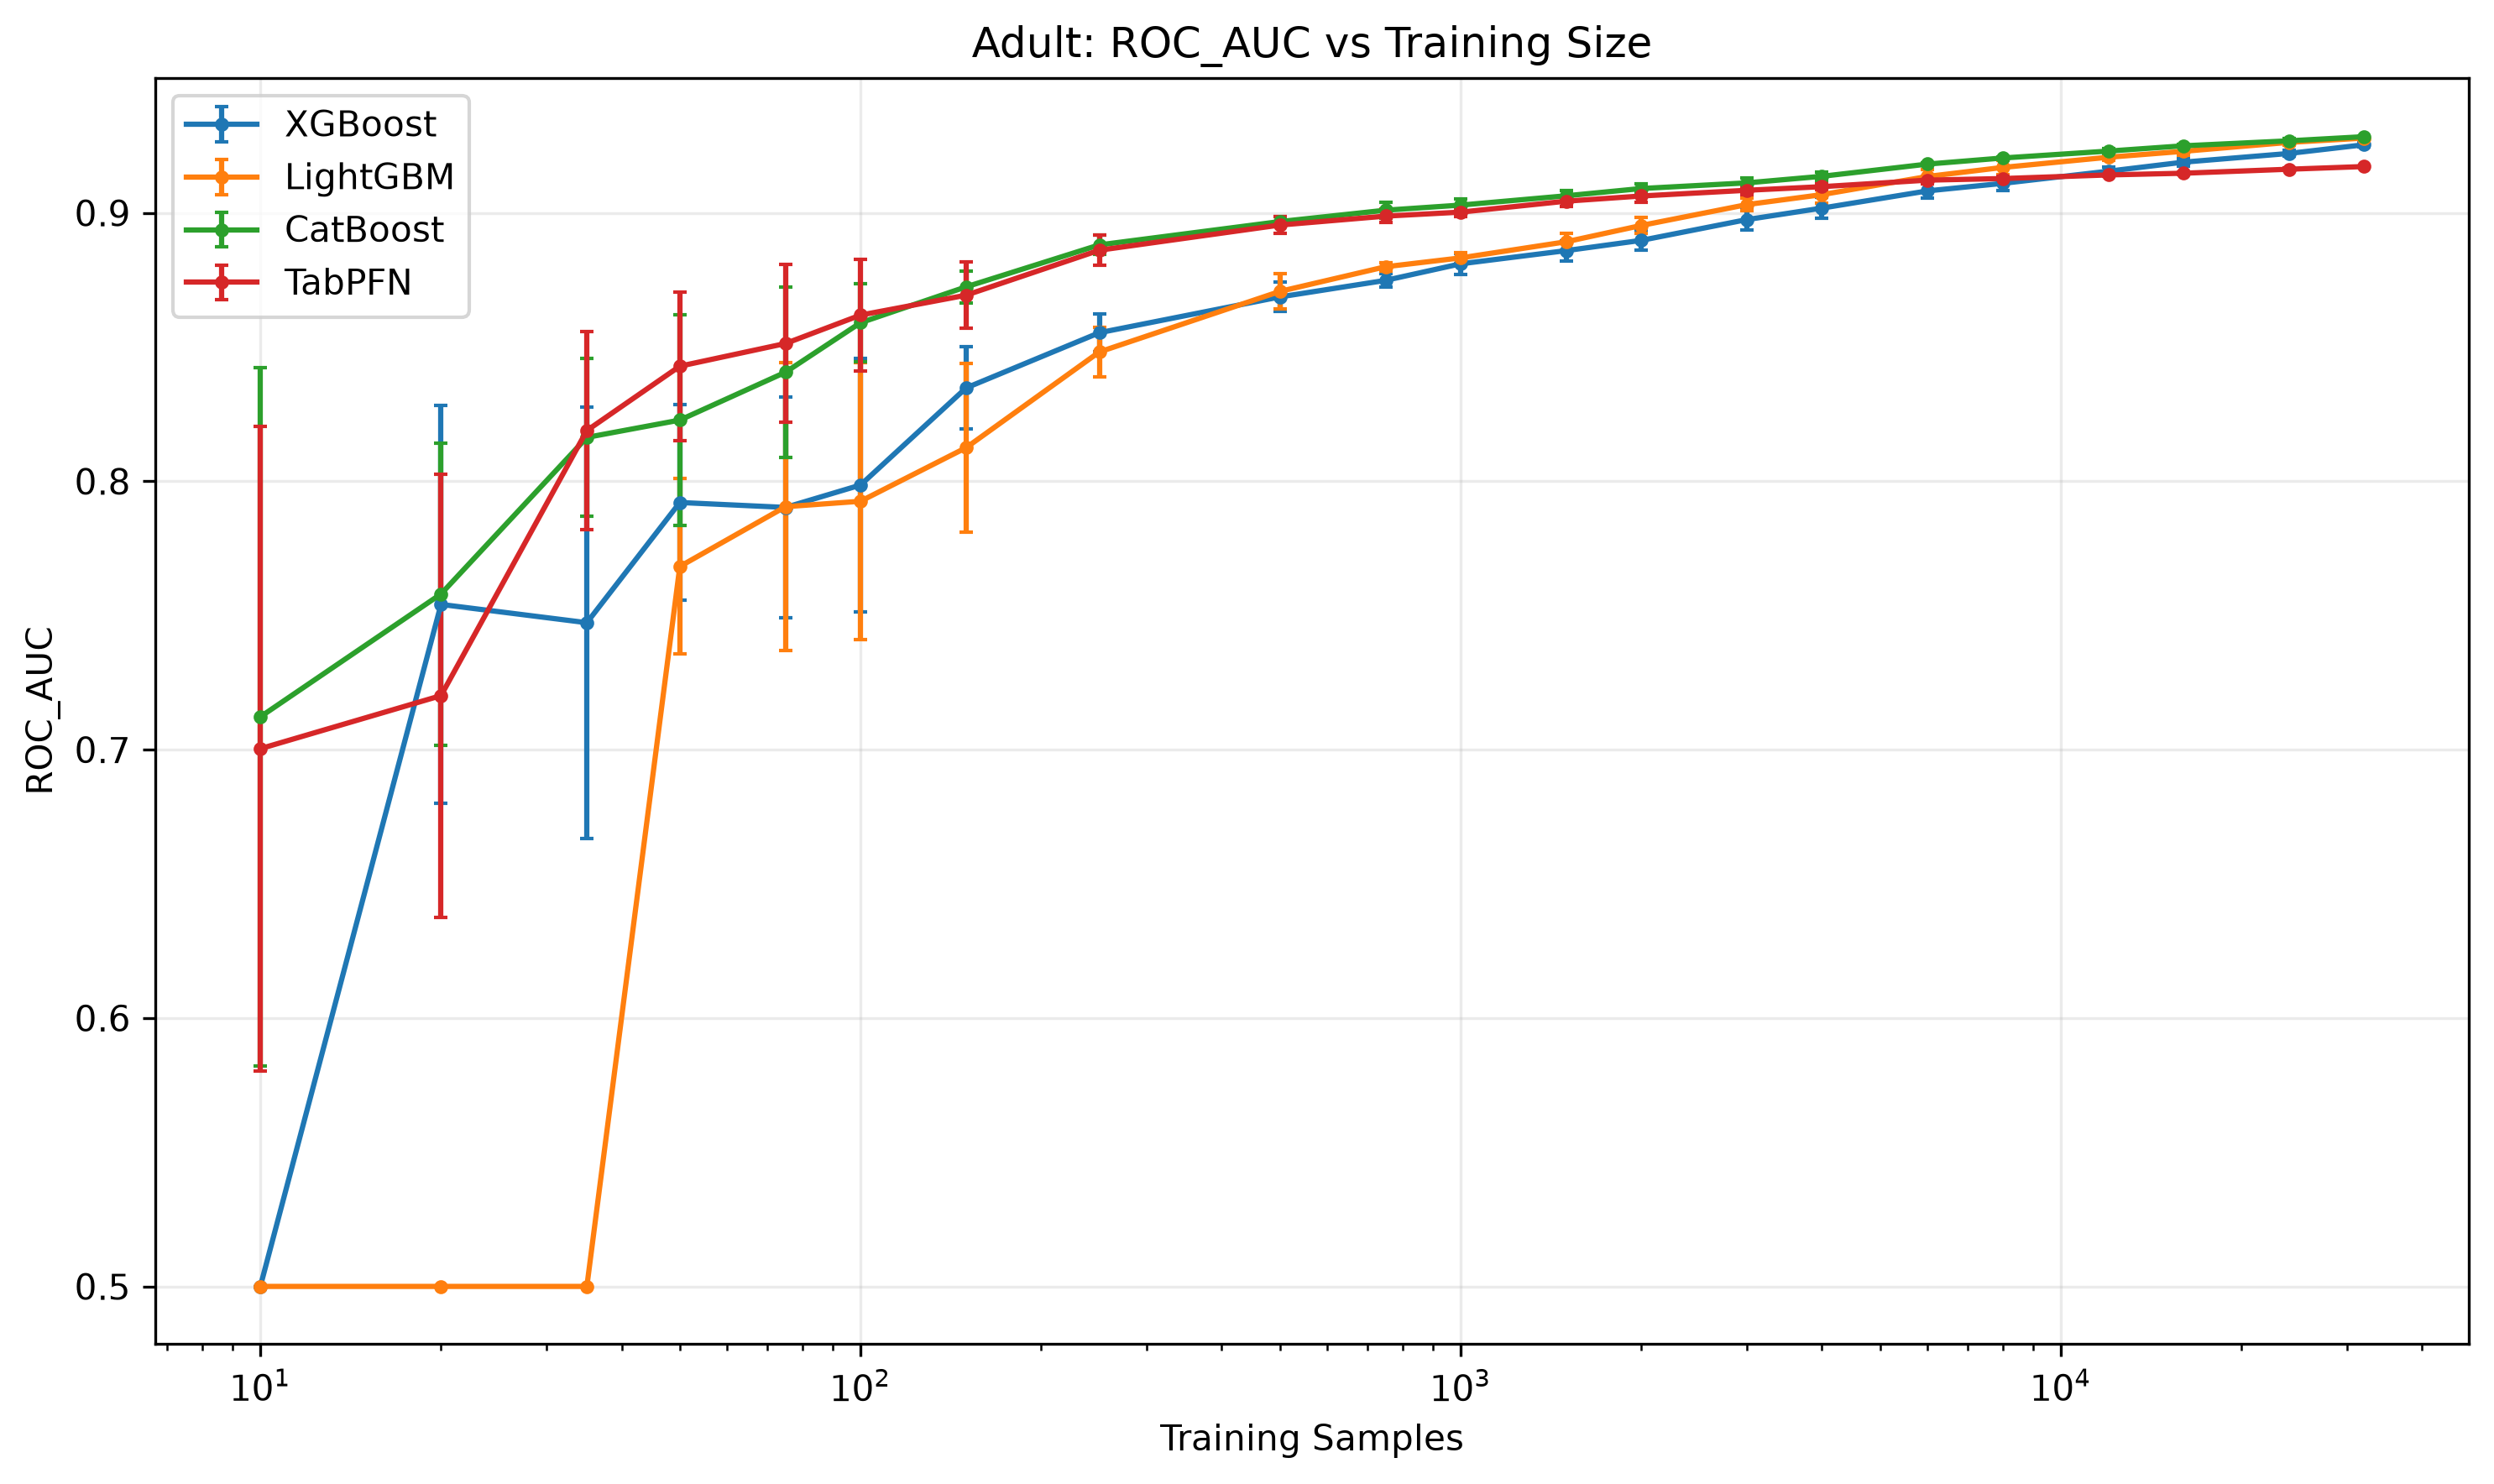
\includegraphics[width=\linewidth]{figures/adult_roc_auc_learning_curve.png}
  \caption{Adult ROC-AUC learning curve.}
  \label{fig:adult-roc-auc}
\end{figure}

\begin{figure}[htbp]
  \centering
  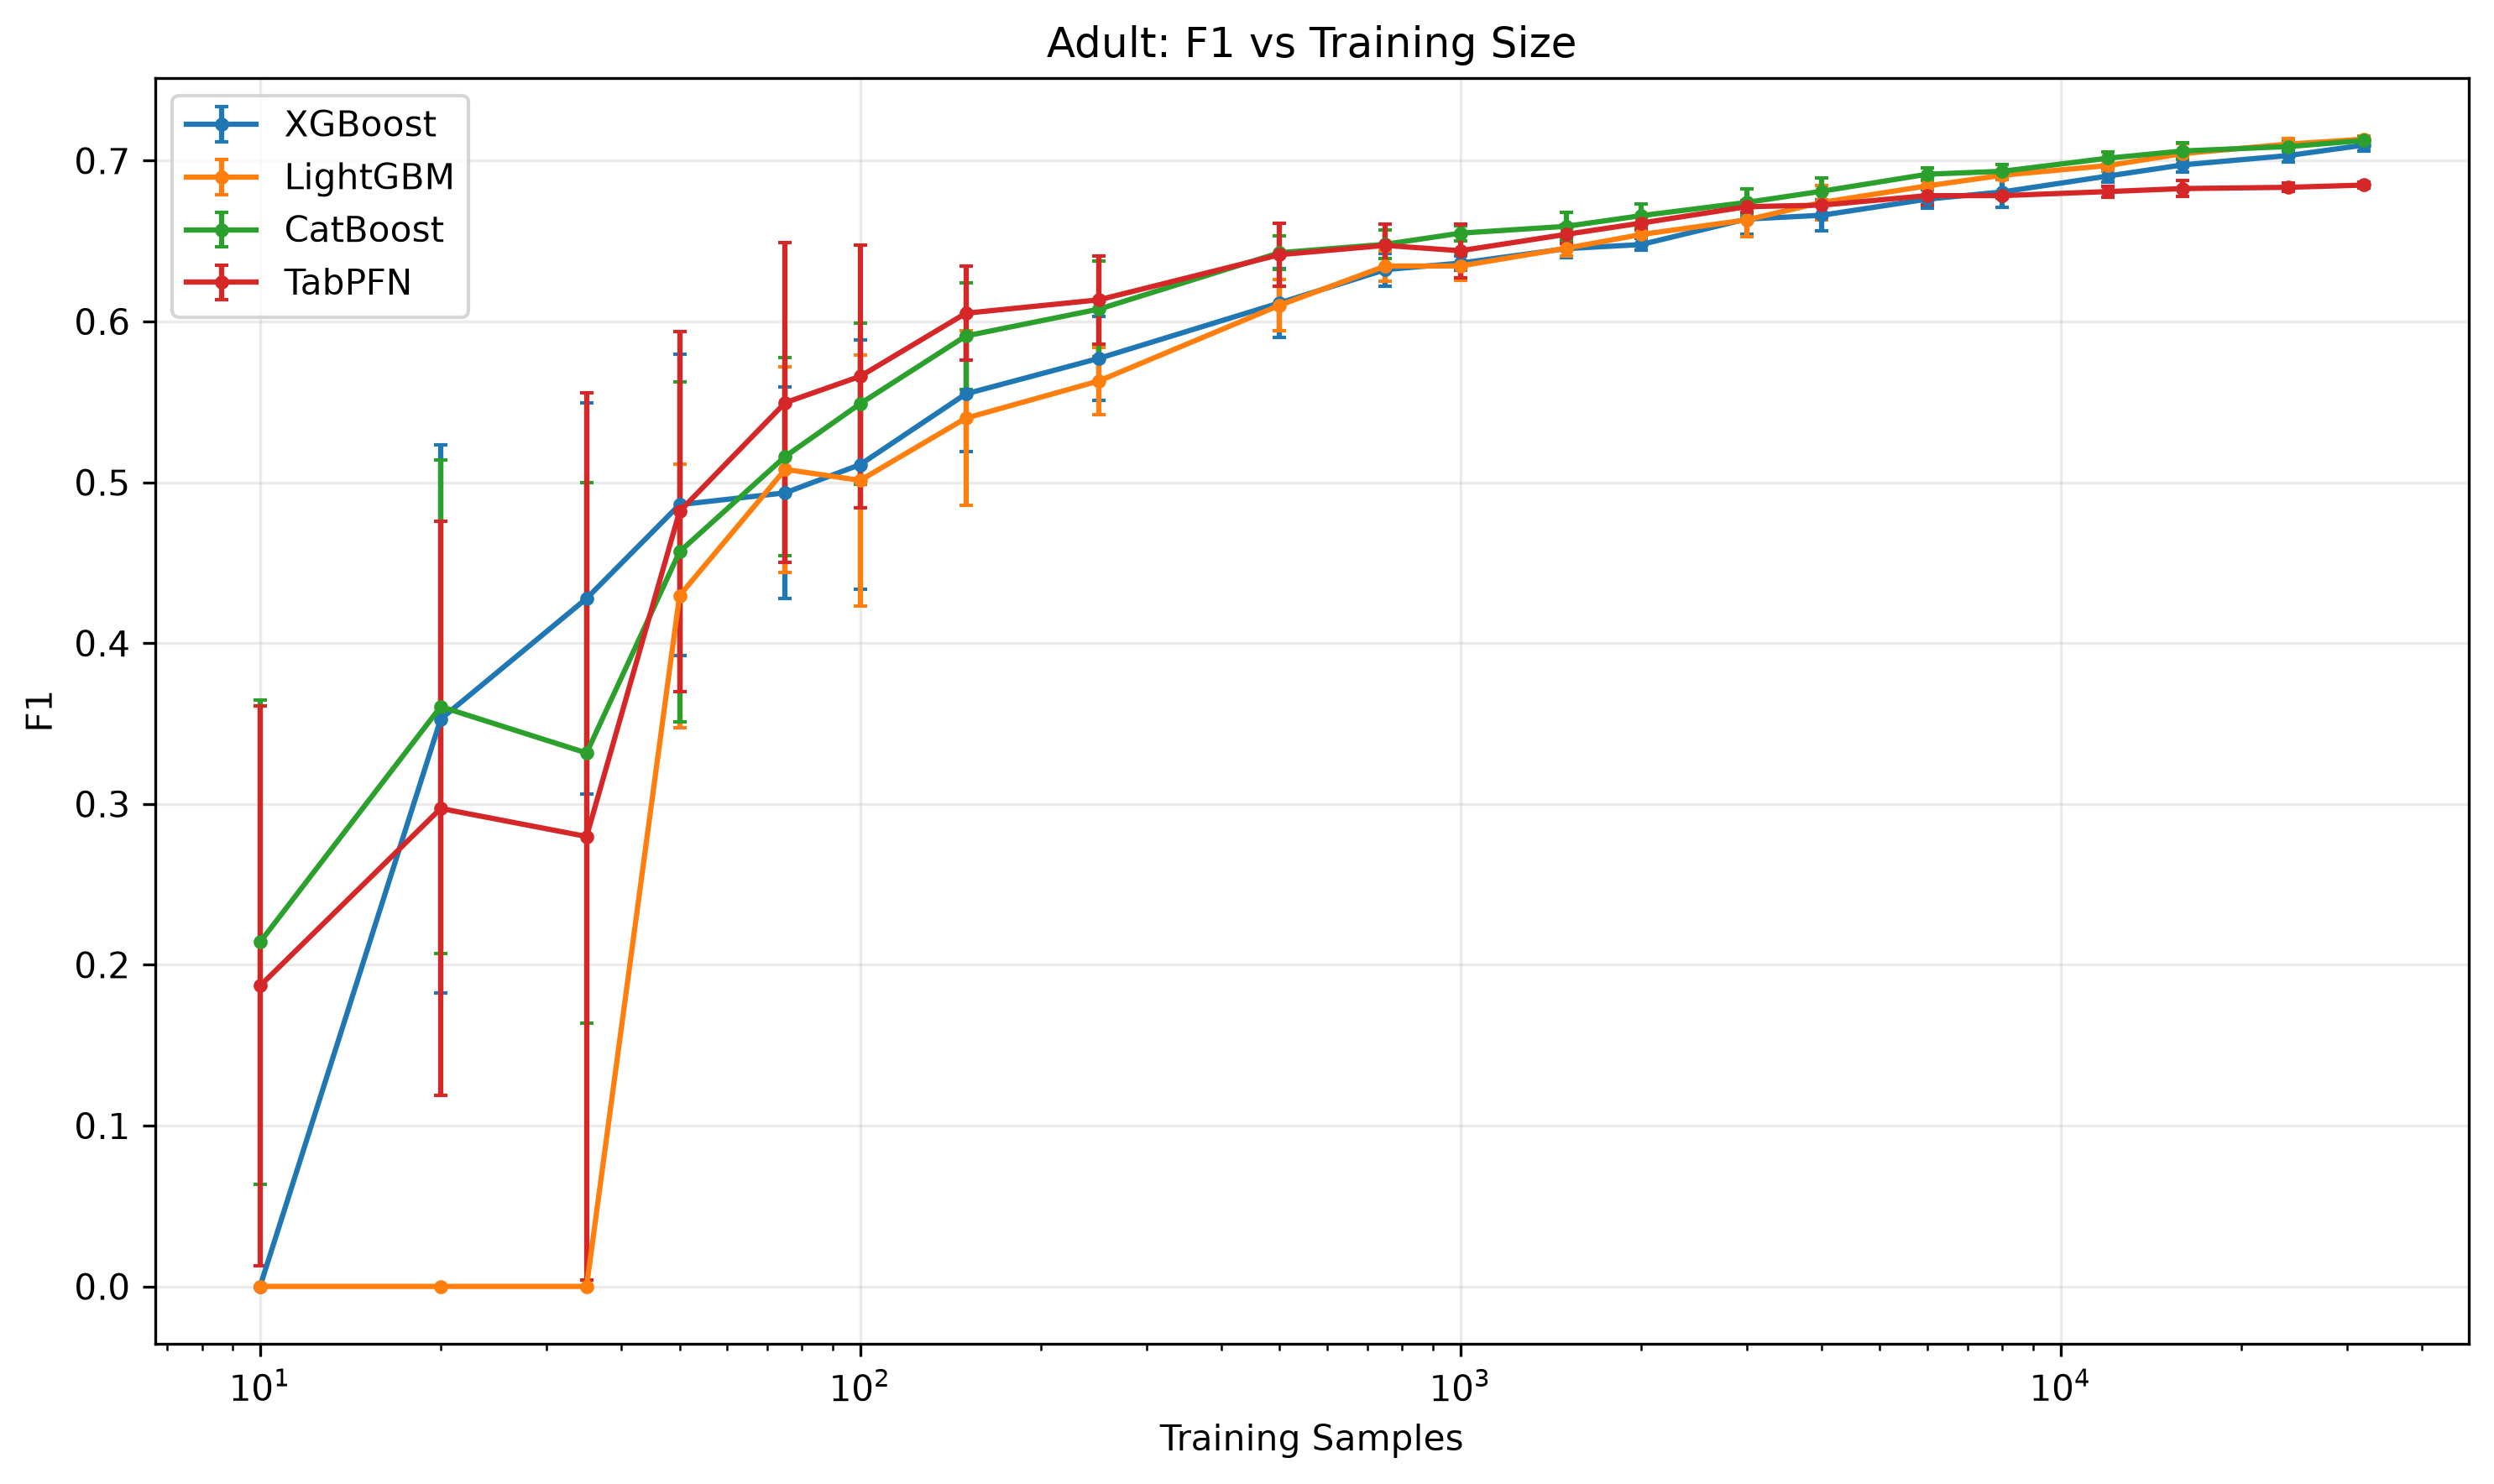
\includegraphics[width=\linewidth]{figures/adult_f1_learning_curve.png}
  \caption{Adult F1 learning curve.}
  \label{fig:adult-f1}
\end{figure}

\begin{figure}[htbp]
  \centering
  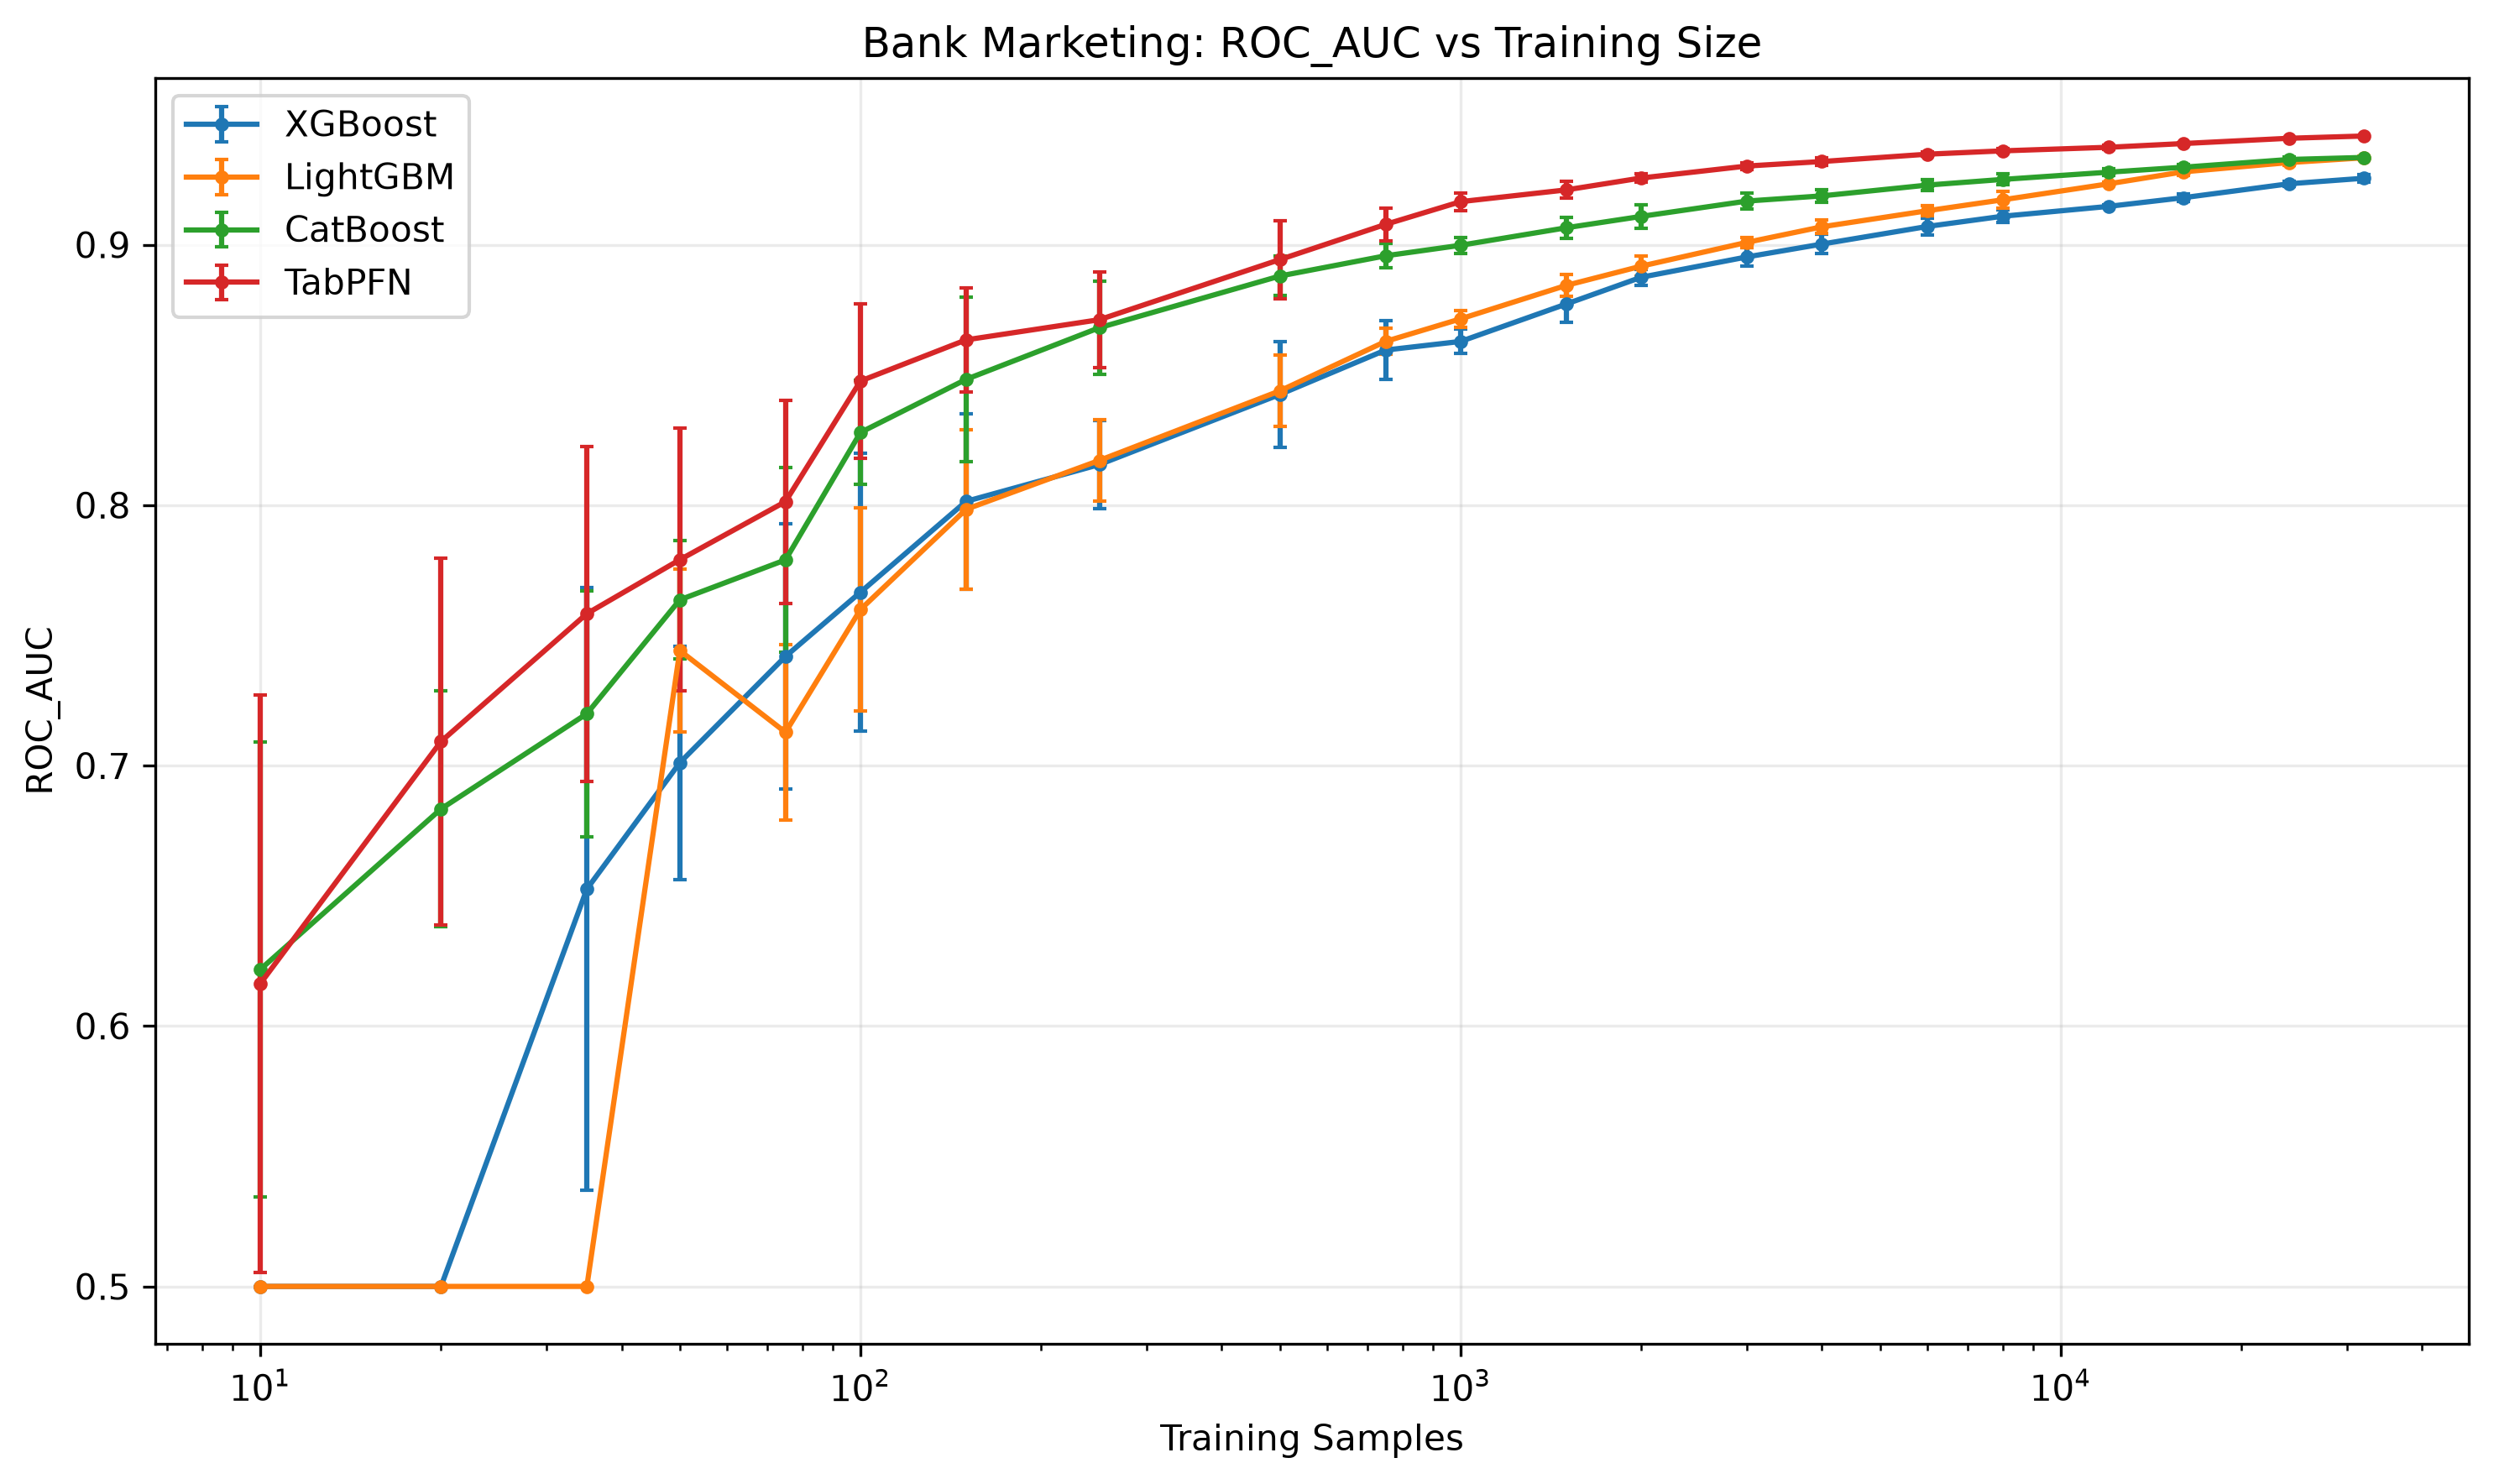
\includegraphics[width=\linewidth]{figures/bank_marketing_roc_auc_learning_curve.png}
  \caption{Bank Marketing ROC-AUC learning curve.}
  \label{fig:bank-roc-auc}
\end{figure}

\begin{figure}[htbp]
  \centering
  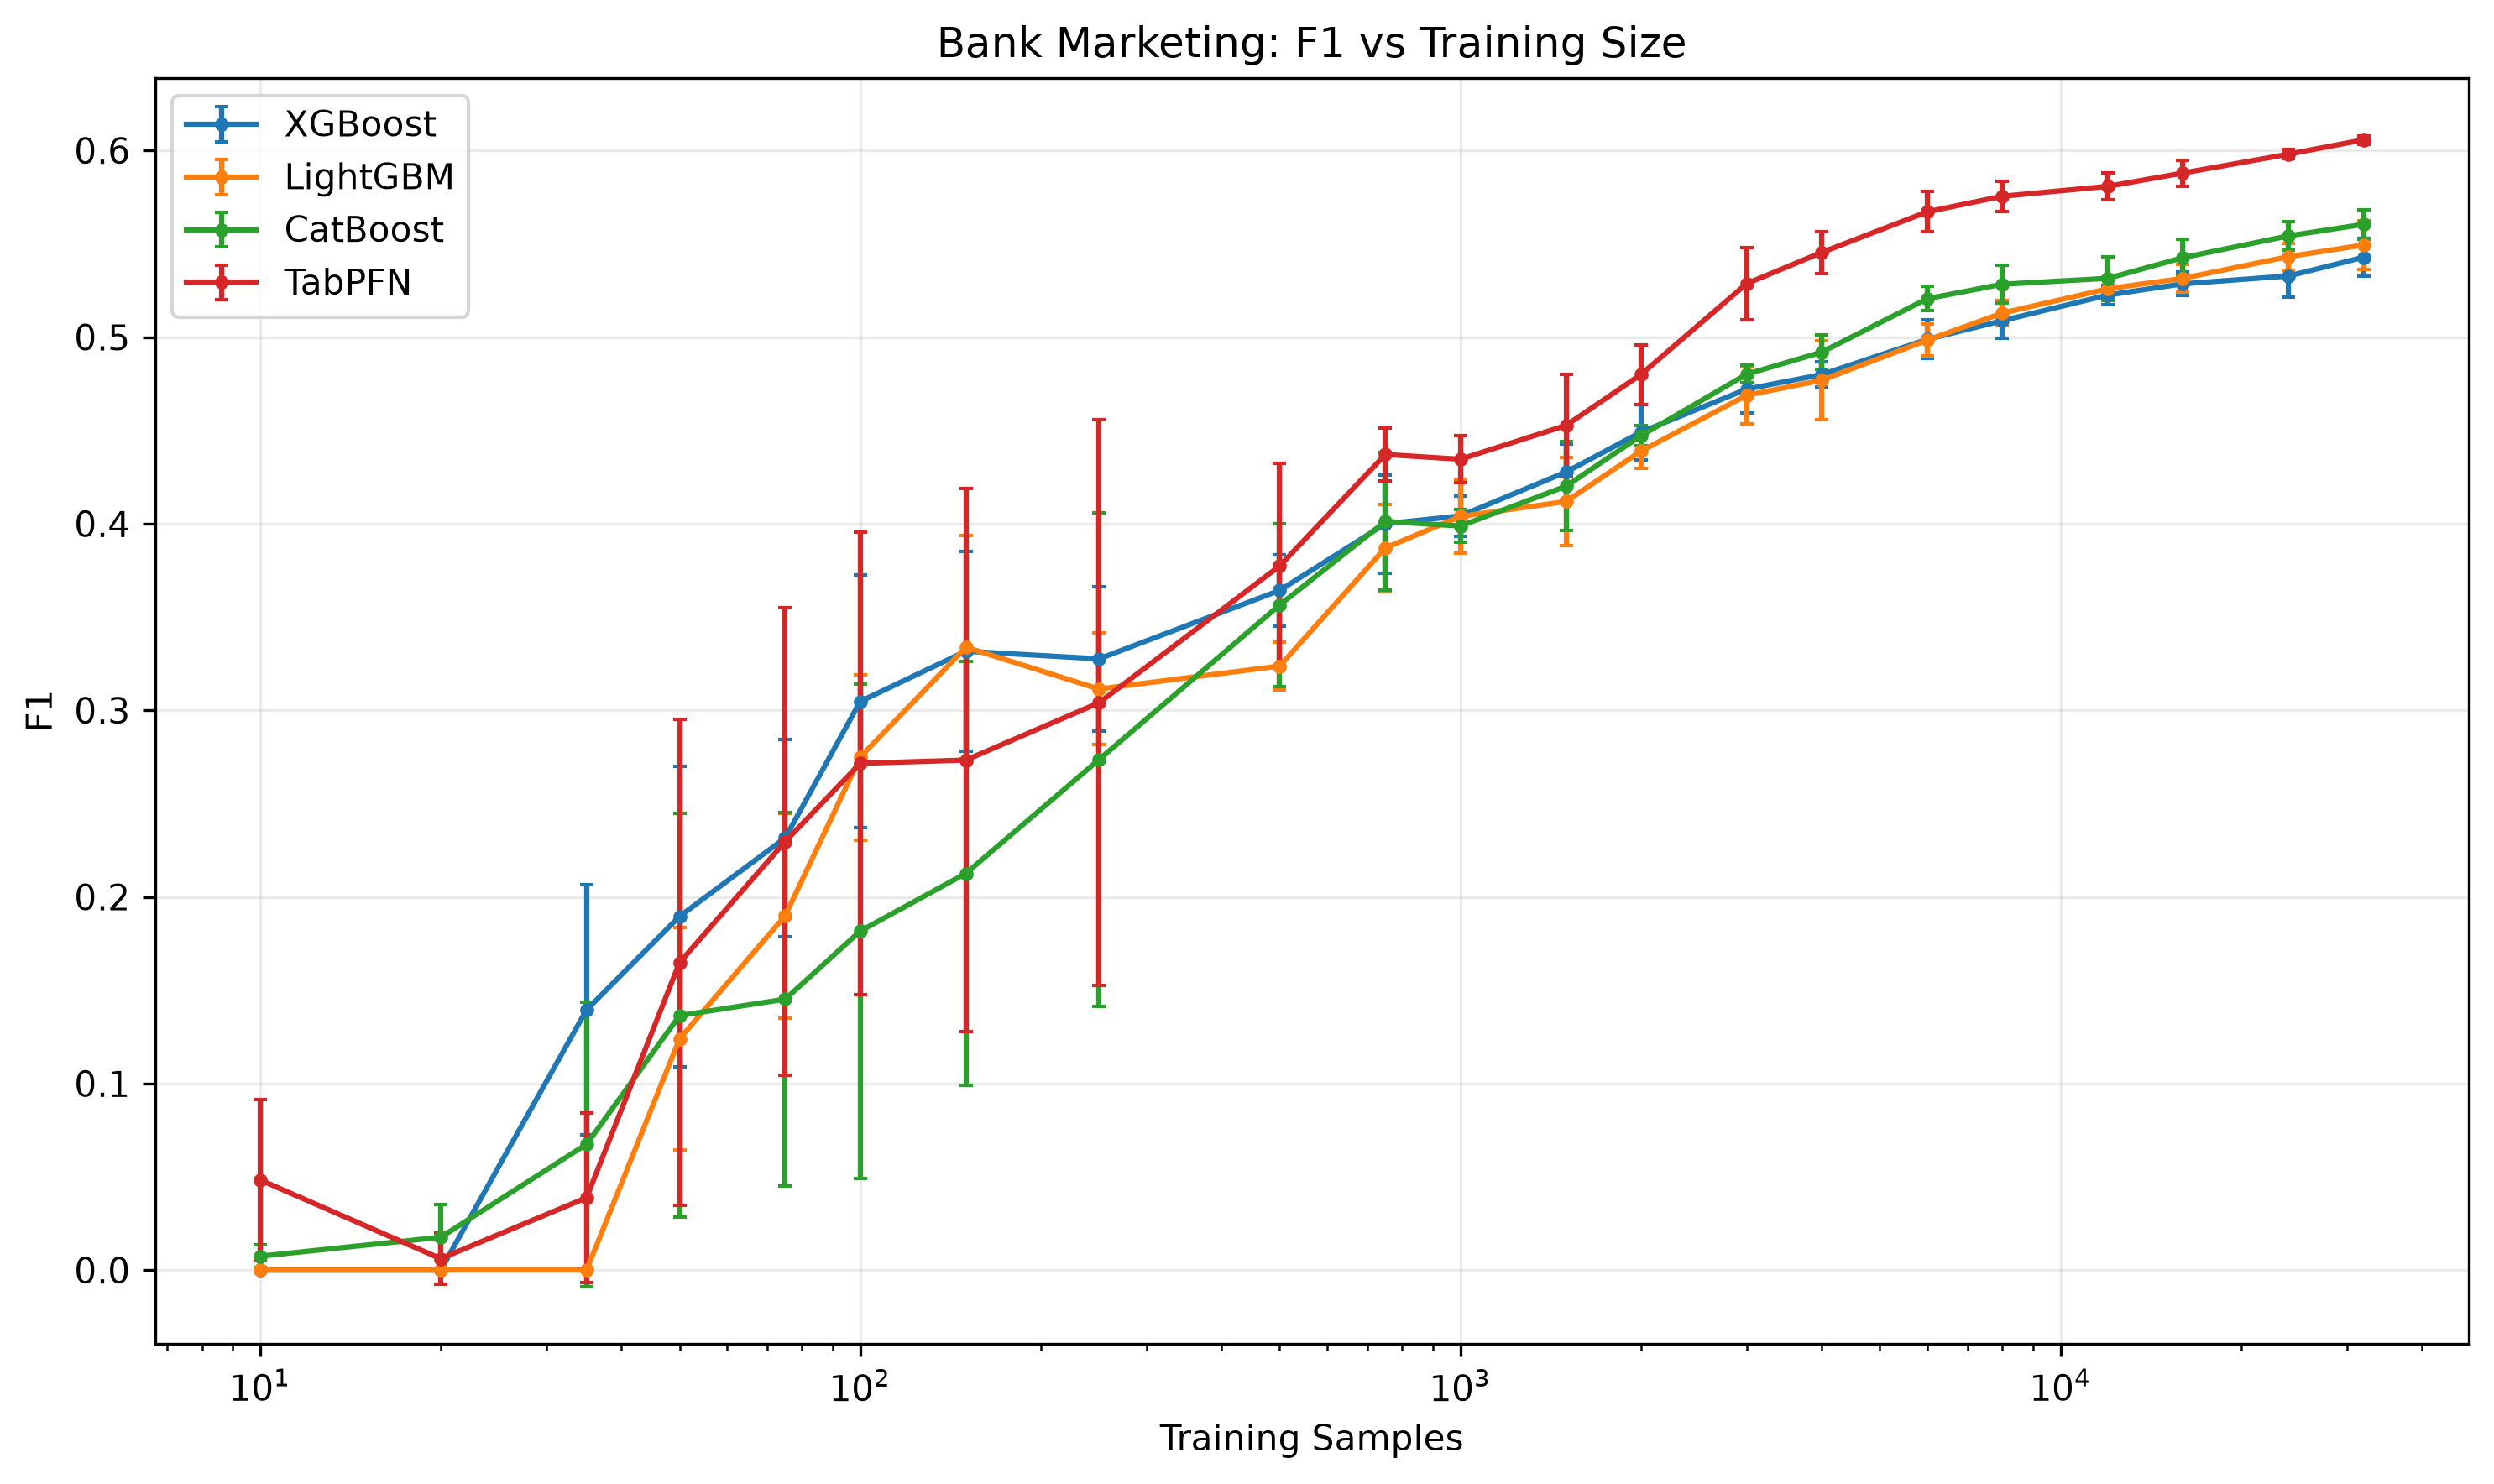
\includegraphics[width=\linewidth]{figures/bank_marketing_f1_learning_curve.png}
  \caption{Bank Marketing F1 learning curve.}
  \label{fig:bank-f1}
\end{figure}

\begin{figure}[htbp]
  \centering
  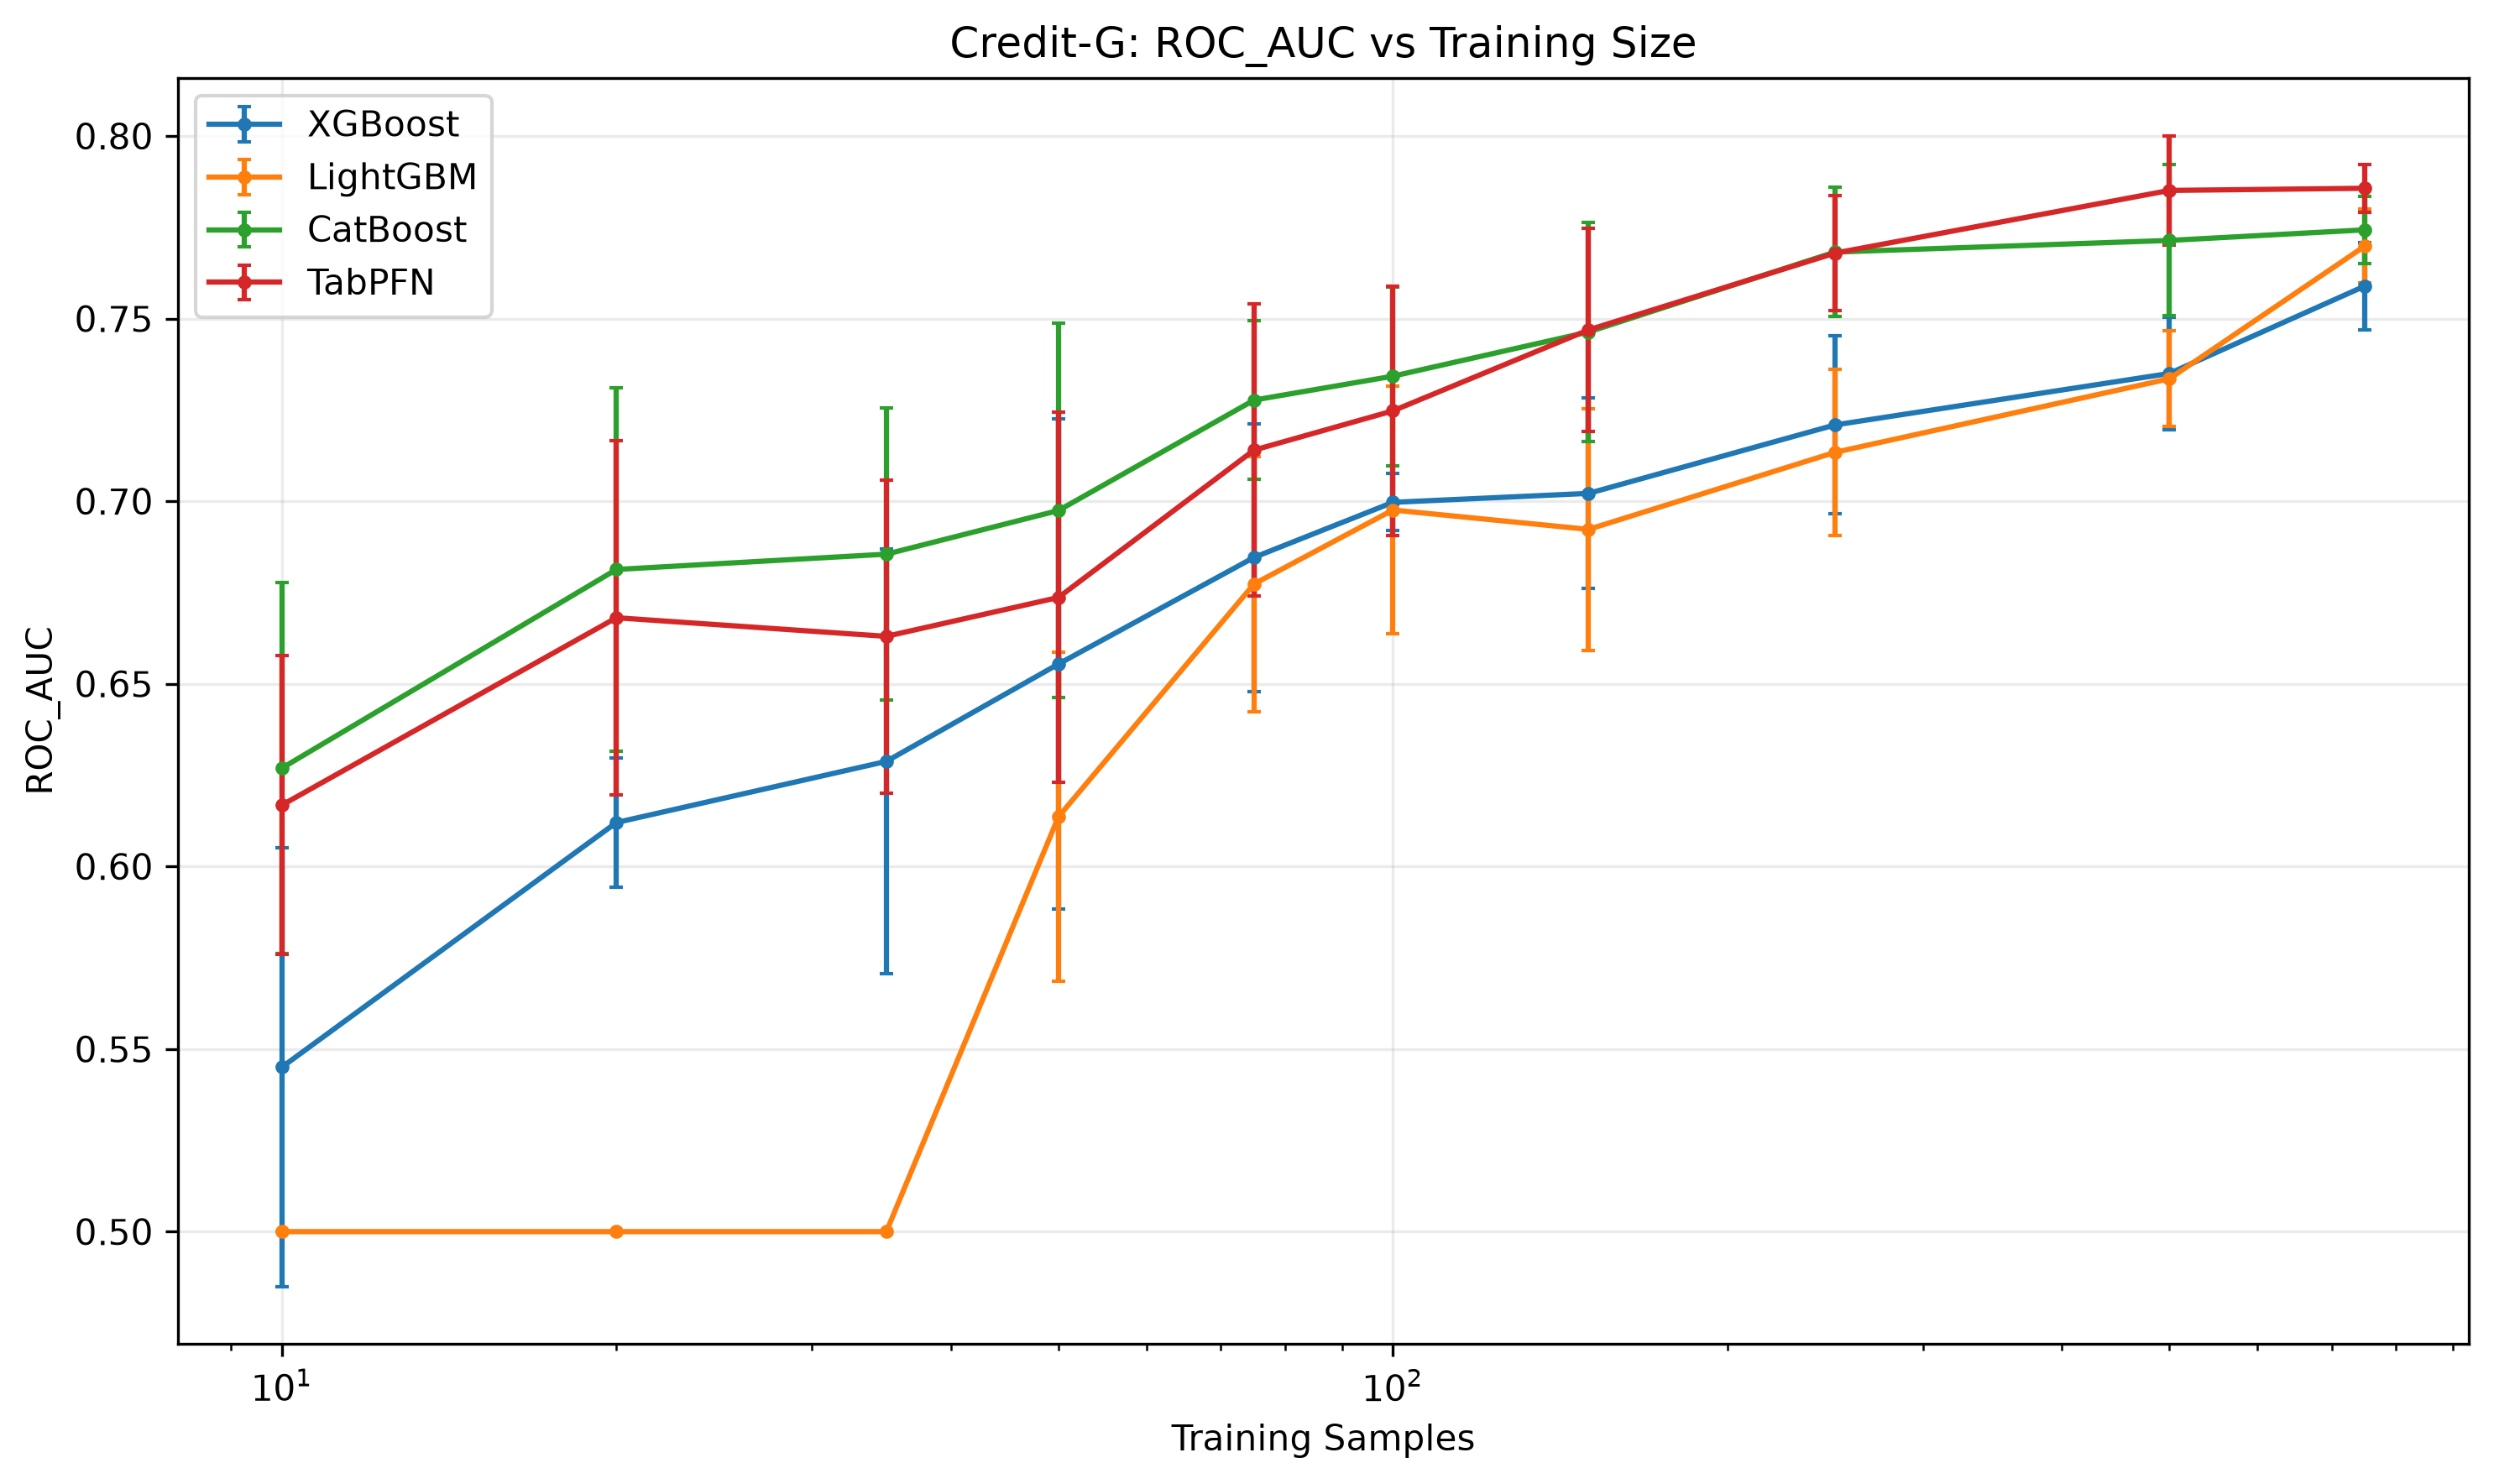
\includegraphics[width=\linewidth]{figures/credit-g_roc_auc_learning_curve.png}
  \caption{Credit-G ROC-AUC learning curve.}
  \label{fig:credit-roc-auc}
\end{figure}

\begin{figure}[htbp]
  \centering
  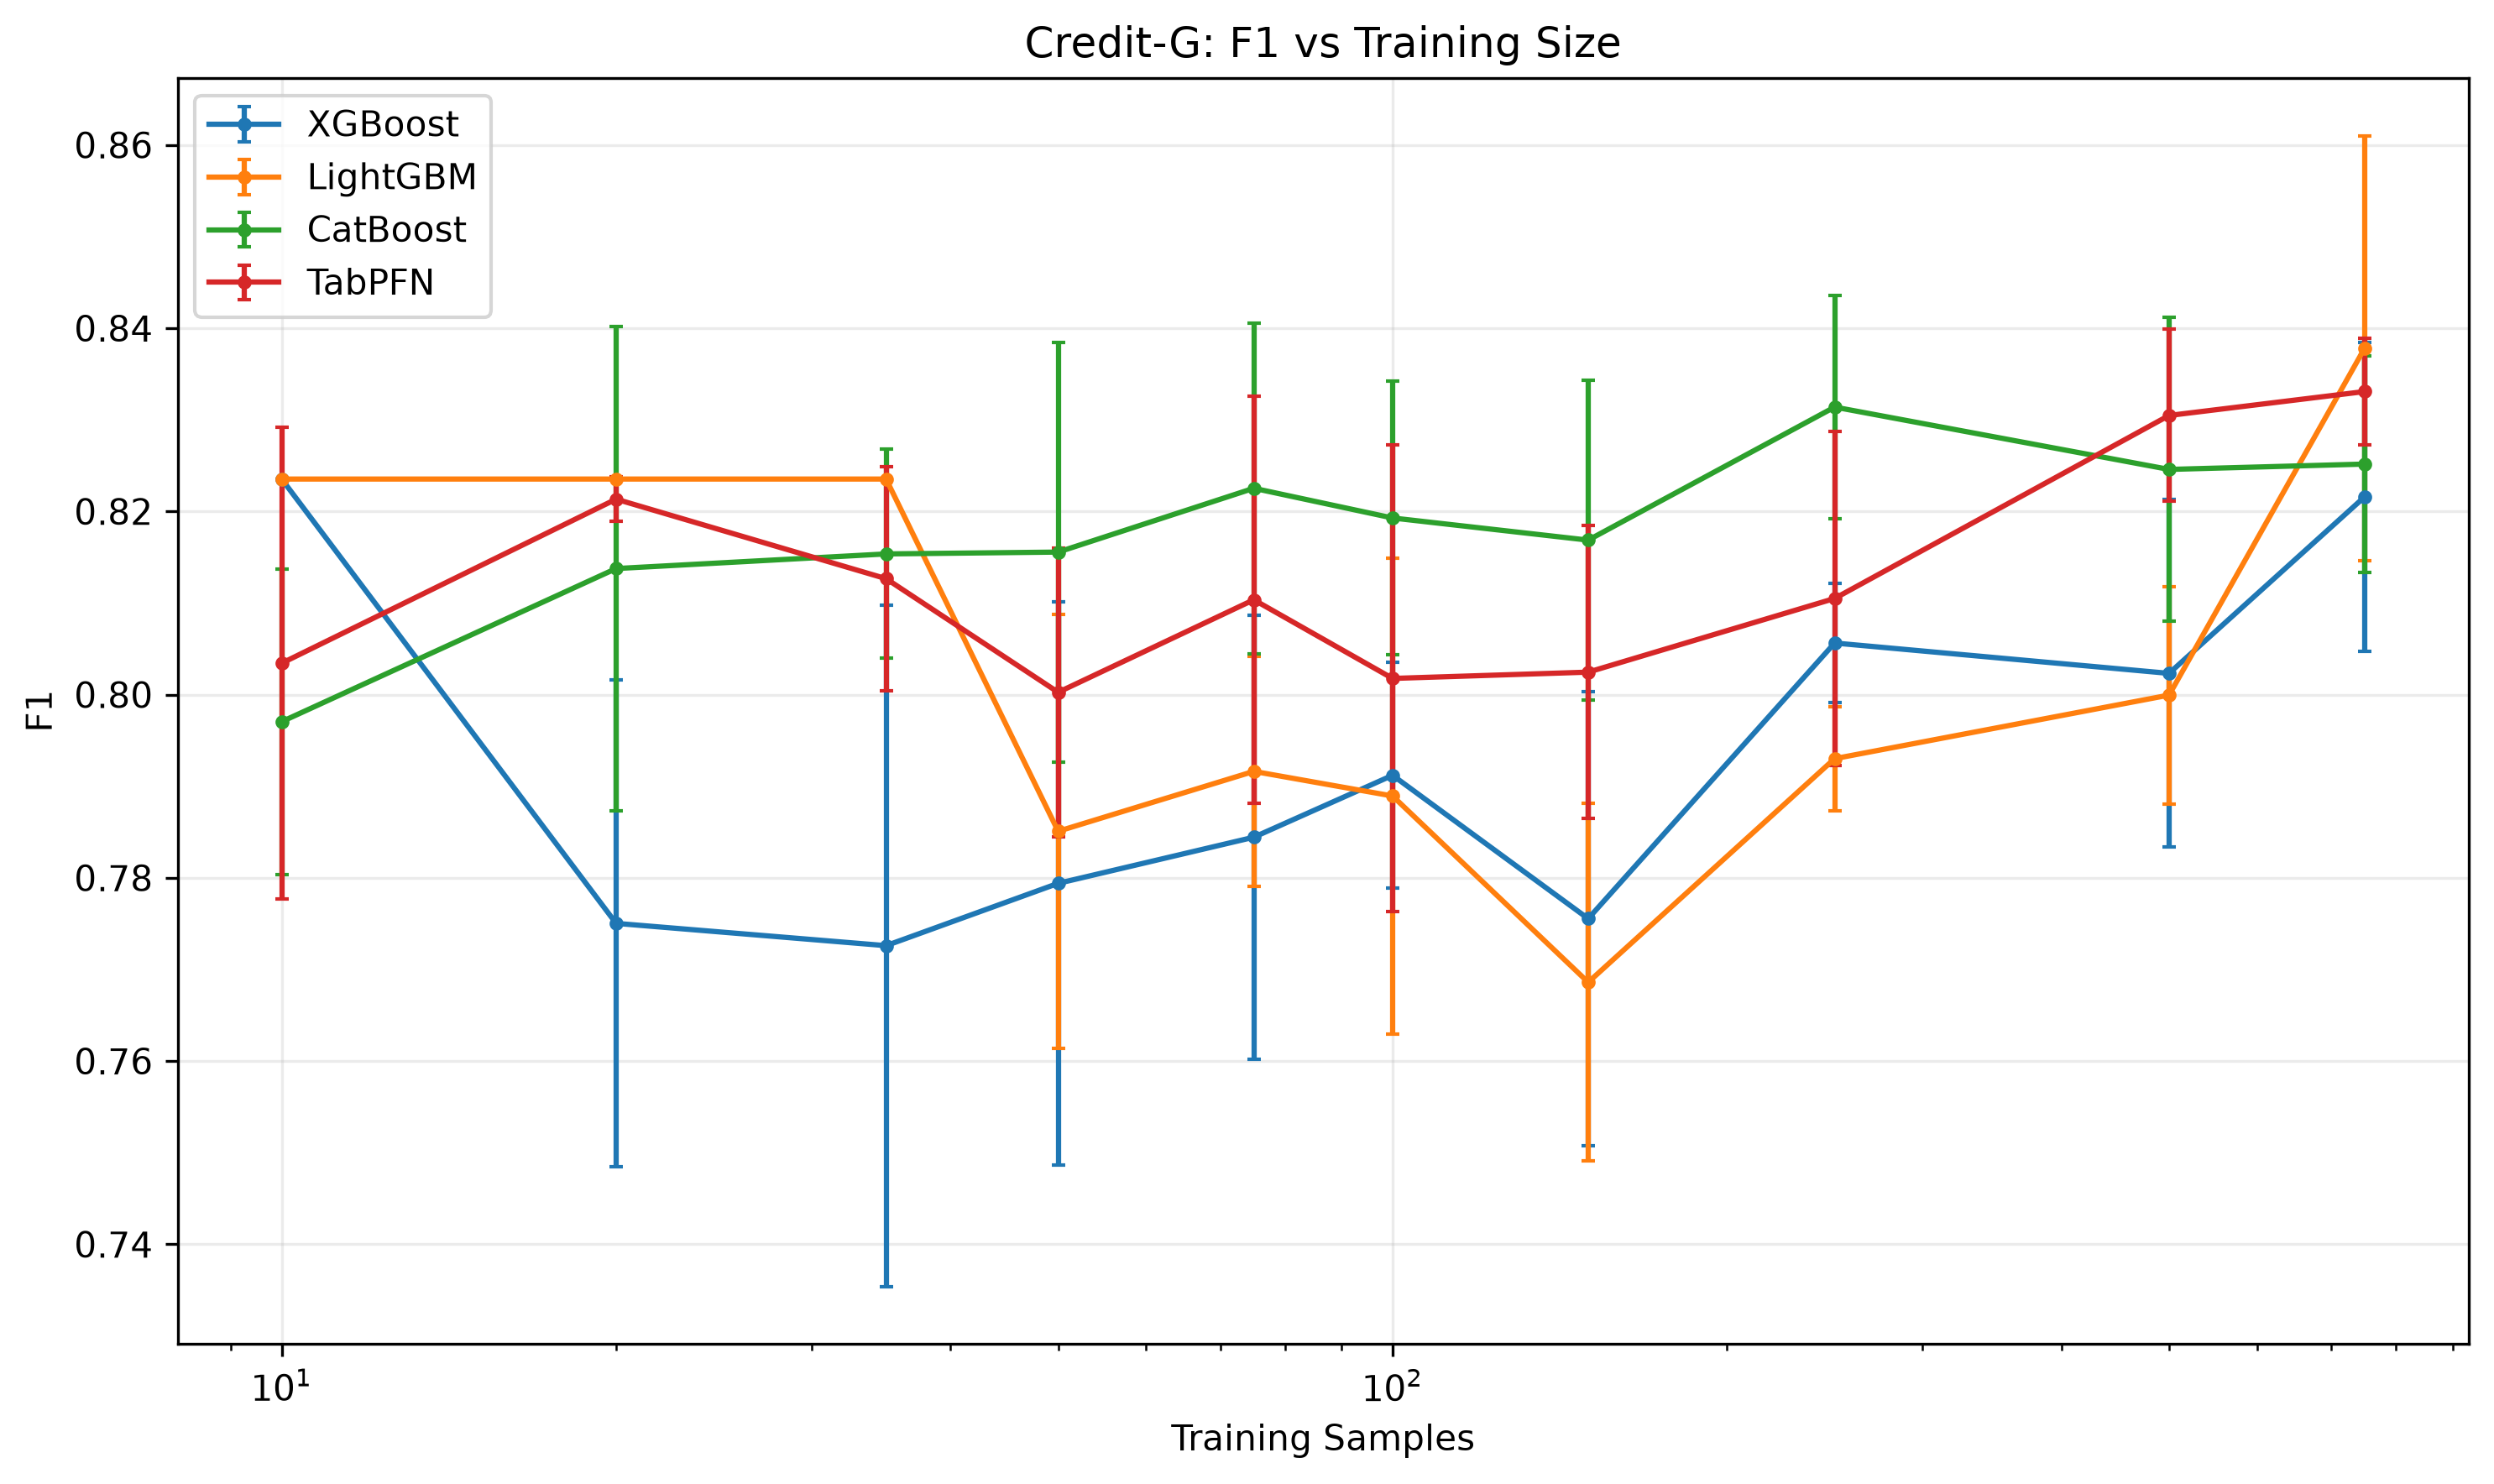
\includegraphics[width=\linewidth]{figures/credit-g_f1_learning_curve.png}
  \caption{Credit-G F1 learning curve.}
  \label{fig:credit-f1}
\end{figure}

\section{Discussion}



\subsection{Overview of the Findings}



The objective of this study was to examine how TabPFN compares with established gradient-boosted tree algorithms across different training-data regimes. The results show that the answer depends on the dataset, evaluation metric, and amount of available training data.



The experiments do not support a general claim that TabPFN is superior to gradient-boosted tree models. Instead, they demonstrate that TabPFN can provide substantial predictive advantages under some conditions while conventional tree-based models remain highly competitive under others.



The clearest advantage for TabPFN was observed on Bank Marketing. In contrast, CatBoost was the strongest overall model on Adult and Credit-G. This variation is important because it demonstrates that model selection for tabular classification cannot be reduced to choosing a single algorithm based solely on its model family.



The results also reveal an important computational trade-off. TabPFN achieved strong predictive performance in several settings but required considerably more prediction time than the conventional tree-based models in this benchmark.



\subsection{Research Question 1: Does TabPFN Provide an Advantage When Training Data Are Limited?}



The results provide partial support for this question.



TabPFN performs strongly in the lower-data regimes, particularly when compared with XGBoost and LightGBM. This pattern is visible on Adult, Bank Marketing, and Credit-G.



For Adult, TabPFN achieves a mean small-regime ROC-AUC of 0.7993, compared with 0.7304 for XGBoost and 0.6419 for LightGBM. However, CatBoost remains slightly stronger at 0.8015.



For Bank Marketing, the difference is considerably larger. TabPFN achieves a small-regime ROC-AUC of 0.7520, compared with 0.6437 for XGBoost and 0.6195 for LightGBM.



Credit-G provides another example of strong TabPFN performance against XGBoost and LightGBM, although CatBoost remains competitive.



Therefore, the findings support the idea that TabPFN can be particularly competitive when labelled training data are limited. However, the results do not establish that TabPFN is always the best model in low-data settings because CatBoost remains highly competitive, particularly on Adult and Credit-G.



\subsection{Research Question 2: How Does TabPFN's Relative Performance Change as Training Size Increases?}



The results do not support a single universal pattern.



On Adult, TabPFN is highly competitive in smaller and medium training regimes, but CatBoost becomes stronger at larger training sizes. In the large regime, CatBoost achieves a mean ROC-AUC of 0.9182 compared with 0.9116 for TabPFN.



This behaviour is consistent with the possibility that conventional gradient-boosted trees can increasingly exploit additional task-specific training observations.



However, Bank Marketing provides an important counterexample. TabPFN maintains an advantage across the small, medium, and large regimes. Its mean ROC-AUC increases from 0.7520 in the small regime to 0.8907 in the medium regime and 0.9339 in the large regime. In the large regime, this remains higher than the corresponding values for XGBoost, LightGBM, and CatBoost.



Consequently, the results do not support a simple hypothesis that TabPFN's advantage necessarily disappears as more training data become available.



Instead, the effect of training-data size is dataset-dependent.



This is an important finding for the study because it indicates that the usefulness of TabPFN cannot be characterized only by the quantity of available training data. Dataset characteristics also appear to influence whether the model retains an advantage at larger training sizes.



\subsection{Research Question 3: Is the TabPFN Advantage Consistent Across Datasets and Metrics?}



The answer is clearly no.



The aggregate results demonstrate substantial differences between datasets.



On Adult, CatBoost is the strongest model across most aggregate metrics. TabPFN remains competitive and performs particularly strongly relative to XGBoost and LightGBM, but it does not achieve the best overall results.



On Bank Marketing, TabPFN is the strongest model across Accuracy, Recall, F1-score, and ROC-AUC, with CatBoost leading only in Precision.



On Credit-G, CatBoost is again the strongest model across most aggregate metrics, while XGBoost achieves the highest Precision.



The statistical analysis reinforces this dataset dependence. Of the 45 paired TabPFN-versus-tree comparisons, 34 are statistically significant at the unadjusted 0.05 level and 31 remain significant after Holm correction. However, significant differences occur in both directions depending on the dataset and baseline.



For example, TabPFN significantly outperforms CatBoost on several Bank Marketing metrics, while it significantly underperforms CatBoost on several Adult metrics. On Credit-G, none of the five TabPFN-CatBoost comparisons is statistically significant.



These findings support H3: the relative performance of TabPFN varies across datasets and evaluation metrics.



This also demonstrates why reporting only an overall average across datasets would be insufficient. Such an aggregate result could hide substantial differences in model behaviour between individual datasets.



\subsection{Research Question 4: What Computational Trade-offs Exist?}



The computational results reveal a clear trade-off between predictive performance and execution time.



TabPFN has the highest mean training time across all three datasets in this benchmark. Its mean training time is approximately 0.679 seconds on Adult, 0.685 seconds on Bank Marketing, and 0.659 seconds on Credit-G.



The difference becomes substantially larger for prediction time.



On Adult, TabPFN requires approximately 9.036 seconds for prediction compared with less than 0.1 seconds for each of the three tree-based models. A similar pattern occurs on Bank Marketing, where TabPFN requires approximately 8.946 seconds compared with approximately 0.04–0.09 seconds for the tree models.



Credit-G shows the same direction, although the absolute difference is smaller: TabPFN requires approximately 0.667 seconds compared with approximately 0.01 seconds for the tree-based models.



Therefore, the predictive advantages observed for TabPFN, particularly on Bank Marketing, are accompanied by a substantial prediction-time cost in this implementation.



This finding is important from a practical perspective. If predictive performance is the primary objective and the additional computation is acceptable, TabPFN may be attractive for some tasks. However, applications requiring very low inference latency may favour conventional tree-based models even when their predictive performance is slightly lower.



The computational results therefore support H4: differences in predictive performance are accompanied by meaningful computational trade-offs.



\subsection{Interpretation of the Model Differences}



The results suggest that TabPFN and gradient-boosted tree models should not be viewed simply as competing implementations of the same learning strategy.



The tree-based models learn a task-specific ensemble from the available observations. Their performance can therefore benefit directly from additional task-specific training data.



TabPFN follows a different paradigm by applying a pretrained model to a new tabular task. Its strong performance in several low- and medium-data configurations is consistent with the potential value of information acquired during pretraining when relatively little task-specific data are available.



However, the results also show that pretraining does not eliminate dataset dependence. CatBoost remains highly competitive on Adult and Credit-G, while TabPFN performs particularly strongly on Bank Marketing.



The differences between datasets therefore suggest that the usefulness of a pretrained tabular model depends on more than sample size alone. Feature characteristics, class distributions, and the relationship between predictors and target may all influence the relative suitability of the approaches.



The present benchmark does not isolate these individual dataset characteristics experimentally, so causal conclusions about why one dataset favours a particular model cannot be established from the current results. Nevertheless, the observed variation provides evidence that dataset-specific behaviour is an important consideration when selecting between tabular foundation models and gradient-boosted trees.



\subsection{Implications for Model Selection}



The results have several practical implications.



First, TabPFN should not automatically replace established gradient-boosted tree models. CatBoost achieves the strongest aggregate performance on two of the three datasets, demonstrating that conventional methods remain highly competitive.



Second, TabPFN should not be dismissed simply because tree-based models are strong baselines. Bank Marketing demonstrates that TabPFN can provide meaningful improvements across several predictive metrics and training-data regimes.



Third, model selection should consider the objective of the application. If predictive discrimination is the primary concern and the additional computational cost is acceptable, TabPFN may be a strong candidate. If inference speed is important, the considerably lower prediction times of the tree-based models may be an important practical advantage.



Finally, the results suggest that evaluating a model at a single training size is insufficient for understanding its practical behaviour. Learning curves reveal changes in relative performance that cannot be observed from a single aggregate benchmark point.



\subsection{Evaluation of the Hypotheses}



\subsubsection{H1: TabPFN will be competitive or superior when training data are limited.}



\textbf{Partially supported.}



TabPFN performs strongly in the smaller training regimes and outperforms XGBoost and LightGBM on several low-data comparisons. However, CatBoost remains competitive or superior on some datasets, particularly Adult and Credit-G.



Therefore, the results support the competitiveness of TabPFN in low-data settings but do not establish universal superiority.



\subsubsection{H2: TabPFN's relative advantage will change as training size increases.}



\textbf{Partially supported.}



The Adult results show a change in relative performance, with CatBoost becoming stronger at larger training sizes. However, Bank Marketing does not follow this pattern because TabPFN maintains its advantage across the evaluated training regimes.



The appropriate conclusion is therefore that training-data size influences relative model performance, but the direction and magnitude of the effect depend on the dataset.



\subsubsection{H3: TabPFN's performance relative to tree models will vary across datasets and metrics.}



\textbf{Supported.}



This is the clearest finding of the study. Adult, Bank Marketing, and Credit-G produce substantially different performance patterns, and the best model varies across evaluation metrics.



The statistical comparisons further demonstrate that the direction of model differences changes according to the dataset and baseline.



\subsubsection{H4: Predictive advantages will involve computational trade-offs.}



\textbf{Supported.}



TabPFN provides strong predictive performance in several settings but has substantially higher measured prediction times than the tree-based models in this benchmark. The results therefore demonstrate a clear predictive-performance versus computational-cost trade-off.



\subsection{Limitations}



Several limitations should be considered when interpreting the findings.



First, the study evaluates only three datasets. Although Adult, Bank Marketing, and Credit-G provide variation in dataset size and classification characteristics, they cannot represent the full diversity of real-world tabular machine-learning problems.



Second, only one tabular foundation model is evaluated. The findings therefore concern TabPFN specifically and should not automatically be generalized to all tabular foundation models.



Third, the benchmark evaluates binary classification only. The conclusions may not transfer directly to multiclass classification, regression, ranking, or other tabular prediction problems.



Fourth, Credit-G has a substantially smaller training partition than Adult and Bank Marketing. As a result, it could not be evaluated across the same large-data training regimes. Comparisons between datasets should therefore be interpreted with this difference in experimental coverage in mind.



Fifth, the computational measurements are specific to the experimental environment and implementation used for the benchmark. Training and prediction times can depend on hardware, software versions, preprocessing, model configuration, and system load. The reported timings should therefore be interpreted as measurements of this experimental setup rather than universal computational costs.



Finally, the benchmark does not attempt to identify the underlying causal characteristics that make one dataset more favourable to TabPFN than another. The observed dataset-level differences demonstrate that such variation exists, but additional controlled experiments would be required to determine which feature or dataset properties are responsible.



\subsection{Overall Interpretation}



The central finding of this study is that there is no universal winner between TabPFN and gradient-boosted tree algorithms.



TabPFN demonstrates strong predictive capability and provides its clearest advantage on Bank Marketing, where it performs strongly across multiple metrics and training-data regimes. At the same time, CatBoost remains highly competitive and achieves the strongest aggregate results on Adult and Credit-G.



The results therefore support a complementary view of tabular foundation models. TabPFN represents a valuable addition to the set of available tabular-learning methods, particularly when its predictive advantages justify its computational requirements. However, the continued strength of gradient-boosted tree algorithms means that they remain important baselines and practical alternatives.



More broadly, the study demonstrates the importance of evaluating tabular models across multiple training-data regimes rather than relying on a single benchmark configuration. Model rankings can change with training size, and the effect is not necessarily consistent across datasets.



The evidence consequently supports a dataset- and application-dependent approach to model selection. Rather than asking whether TabPFN is universally better than gradient-boosted trees, a more useful practical question is under which conditions the additional capabilities of a tabular foundation model provide sufficient predictive benefit to justify its computational cost.

\section{Conclusion}



This study presented an empirical comparison of TabPFN and three established gradient-boosted tree algorithms—XGBoost, LightGBM, and CatBoost—across different training-data regimes. The benchmark evaluated the models on three binary tabular classification datasets, using five random seeds and multiple training sizes to examine both overall predictive performance and changes in performance as additional training data became available.



The results show that TabPFN can achieve highly competitive predictive performance, but its effectiveness is dataset-dependent. Bank Marketing provided the clearest evidence in favour of TabPFN, where it achieved the highest mean Accuracy, Recall, F1-score, and ROC-AUC and maintained strong performance across the evaluated training-data regimes. In contrast, CatBoost achieved the strongest overall results on Adult and Credit-G, demonstrating that conventional gradient-boosted tree methods remain highly competitive.



The learning-curve analysis further showed that there is no universal relationship between training-set size and TabPFN's relative advantage. On Adult, CatBoost became increasingly competitive at larger training sizes, whereas TabPFN maintained an advantage across the evaluated regimes on Bank Marketing. Credit-G produced an intermediate pattern in which TabPFN remained competitive with the tree-based models but did not consistently outperform CatBoost.



The statistical analysis supports these observations. A substantial proportion of the paired TabPFN-versus-tree comparisons were statistically significant, but the direction of the differences varied across datasets and baseline models. This indicates that statistical evidence for differences between the models should not be interpreted as evidence of universal TabPFN superiority.



The computational results also revealed an important trade-off. Although TabPFN provided strong predictive performance in several settings, it required substantially more prediction time than the conventional tree-based models in the experimental environment. Consequently, model selection should consider both predictive performance and computational requirements.



Overall, the findings suggest that TabPFN should be viewed as a complementary approach to gradient-boosted tree algorithms rather than as a universal replacement. Its advantages are most meaningful when the observed predictive improvements justify the additional computational cost. The results also demonstrate the value of evaluating tabular models across multiple training-data regimes, since model rankings can change as the amount of available training data increases.



Future work could extend the benchmark to a larger and more diverse collection of tabular datasets, include additional tabular foundation models, evaluate multiclass and regression tasks, and investigate which measurable dataset characteristics are associated with stronger or weaker performance from pretrained tabular models. Such extensions would help determine whether the dataset-dependent patterns observed in this study generalize beyond the three datasets considered here.

\printbibliography
\end{document}
